\documentclass[twoside]{ctuthesis}

% extra balíky a jejich nastavení

\usepackage{morewrites}
\usepackage{calc}
\usepackage{todonotes} % todos
\usepackage{blindtext} % lorem
\usepackage{csquotes}  % quotes
\usepackage{wrapfig}

\usepackage{svg}
\svgpath{img/}

\usepackage[all]{nowidow} % fix for orphaned lines of text
\usepackage{fancyvrb}
\usepackage{siunitx}
\usepackage{sectsty}
\usepackage{titlecaps}
\usepackage{cprotect}
\usepackage{framed}
\usepackage{subcaption}

\usepackage{tabularx}
\usepackage{tabulary}
\usepackage{longtable}
\usepackage{tabu} % longtabu

\usepackage{pmboxdraw}

\usepackage{xcolor}
\definecolor{RubineRed}{HTML}{C30067}

\usepackage{flafter} % ensures embeds won't go before their references
\usepackage{enumitem} % better list spacing

\usepackage{bigfoot} % verbatin in footnote
\usepackage{makecell} % cells with custom align in tabular
\usepackage{tabto} % tabs, but kinda buggy
\usepackage{ragged2e} % this was supposed to improve text alignment

\newcommand{\CS}{C\nolinebreak\hspace{-.05em}\raisebox{.4ex}{\scriptsize\bf \#}}

% some symbols. skip integrals because asmmath also defines them and is loaded by the thesis class
\usepackage[nointegrals]{wasysym}

\usepackage[
	style=numeric,
	backend=biber
]{biblatex}

% Uvozovky v češtině
\iffalse
	% makro pro uvozovky
	\renewcommand\uv[1]{\enquote{#1}}
	% \DeclareQuoteStyle{czech}
	 	{\quotedblbase}
	 	{\textquotedblleft}
	 	{\textquoteleft}
	 	{\textquoteright}
\fi

%% MINTED
\usepackage{minted}    % code listings 
\usepackage{xpatch,letltxmacro}
\LetLtxMacro{\cminted}{\minted}
\let\endcminted\endminted
\xpretocmd{\cminted}{\RecustomVerbatimEnvironment{Verbatim}{BVerbatim}{}}{}{}
\newminted{ini}{frame=leftline,autogobble=true}


%% CTUTHESIS CONFIG

\ctusetup{
	xdoctype = M,
	front-list-of-tables = true,
	mainlanguage = english,
	%
	author = {Bc. Ondřej Hruška},
	supervisor = {doc. Ing. Radislav Šmíd, Ph.D.},
	%
	title-english = {Learning and automation GPIO platform},
	title-czech = {Výuková a automatizační GPIO platforma},
	%
	xfaculty = F3,
	department-czech = {Katedra měření},  
	fieldofstudy-czech = {Kybernetika a~robotika},
	subfieldofstudy-czech = {Senzory a~přístrojová technika},
	%
	department-english = {Department of Measurement},
	fieldofstudy-english = {Cybernetics and Robotics},
	subfieldofstudy-english = {Sensors and Instrumentation},
	front-specification = true,
	specification-file = {zadani-zakryto.pdf},
	%specification-file = {zadani-doc.pdf},
	%specification-file = {zadani-doc.pdf},
	%
	keywords-czech = {},
	keywords-english = {},
	%
	day = 0,     % ???
	month = 0,  % ???
	year = 2018, % ???
}

\ctuprocess

\hypersetup{
	pdftitle = {Learning and automation GPIO platform},
	pdfauthor = {Ondřej Hruška}
}

% Extra info na titulní stránce
\addto\ctucaptionsczech{%
	\def\supervisorname{Vedoucí}%
	\def\subfieldofstudyname{Studijní program}%
}

% Abstrakt, poděkování atd
\ctutemplateset{maketitle twocolumn default}{
	\begin{twocolumnfrontmatterpage}
		\ctutemplate{twocolumn.thanks}
		\ctutemplate{twocolumn.declaration}
		\ctutemplate{twocolumn.abstract.in.titlelanguage}
		\ctutemplate{twocolumn.abstract.in.secondlanguage}
		\ctutemplate{twocolumn.tableofcontents}
		\ctutemplate{twocolumn.listoffigures}
	\end{twocolumnfrontmatterpage}
}



%% SPACING

% Booktabs
\setlength{\heavyrulewidth}{0.5mm}
\setlength{\lightrulewidth}{0.25mm}
\setlength{\cmidrulewidth}{0.25mm}

% More space in table cells
\renewcommand{\arraystretch}{1.4}

% Fix overful hbox
\setlength{\emergencystretch}{.5em}

% -- odstavce --
\setlength\parskip{1.5ex plus 1pt minus 1 pt}
%\setlength{\parskip}{1.5ex plus 0.2ex minus 0.1ex} % po změně je potřeba doladit nadpisy
%\renewcommand{\baselinestretch}{1.1}
\setlength\parindent{.5cm}

% add blank page unless current is left
%\newcommand*\cleartoleftpage{%
%	\clearpage
%	\ifodd\value{page}\hbox{}\newpage\fi
%}

% don't clear page before chapter
%\renewcommand{\cleardoublepage}{\clearpage}

% section on new page, except first
%\pretocmd{\section}{%
%	\ifnum\value{section}=0 \else\clearpage\fi
%}{}{}

% ??? what does this do
\makeatletter
\newcommand*{\centerfloat}{%
	\parindent \z@
	\leftskip \z@ \@plus 1fil \@minus \textwidth
	\rightskip\leftskip
	\parfillskip \z@skip}
\makeatother




%% LINK COLORS
\hypersetup{
	colorlinks,
	linkcolor={red!50!black},
	citecolor={blue!50!black},
	urlcolor={blue!80!black}
}

\usepackage{bookmark}
\bookmarksetup{
	numbered,
}

%nice referencing with the words auto generated
\usepackage[nameinlink,capitalize,noabbrev]{cleveref}

%% ACRONYM CONFIG
\usepackage[xindy,nonumberlist,nomain,acronym,nopostdot,toc=false]{glossaries}
%\glssetwidest{ABCD}
\renewcommand*{\glsclearpage}{}
\usepackage{glossary-mcols}
\renewcommand*{\glspostdescription}{}
\makeglossaries
\glsaddall

% make glsosary entries black
%\renewcommand*{\glstextformat}[1]{\textcolor{black}{#1}}


%% HELPER MACROS

\newcommand\nobr[1]{\mbox{#1}}

% monospace
\newcommand\mono[1]{\texttt{#1}}

% library name
\newcommand\lib[1]{\textit{#1}}

% název listing figure
% \renewcommand\listingscaption{Program}

% \newcommand\zdroj[1]{\textit{Zdroj: #1}}


%% UNITS

\newcommand{\uF}{\micro\farad}
\newcommand{\nF}{\nano\farad}
\newcommand{\cm}{\centi\metre}
\newcommand{\VperA}{\V/\A}

\newcommand{\IIC}{I\textsuperscript{2}C\xspace}
\newcommand{\IIS}{I\textsuperscript{2}S\xspace}
\newcommand{\arm}{Arm\xspace}
\newcommand{\armcm}{Arm Cortex-M\xspace}
\newcommand{\mbed}{Arm Mbed\xspace}

\newcommand*\xCmdName[2]{#1~(#2)\xspace}

\newcommand*\CmdSuccess{\xCmdName{0x00}{Success}}
\newcommand*\CmdPing{\xCmdName{0x01}{Ping}}
\newcommand*\CmdError{\xCmdName{0x02}{Error}}
\newcommand*\CmdBulkReadOffer{\xCmdName{0x03}{Bulk~Read~Offer}}
\newcommand*\CmdBulkReadPoll{\xCmdName{0x04}{Bulk~Read~Poll}}
\newcommand*\CmdBulkWriteOffer{\xCmdName{0x05}{Bulk~Write~Offer}}
\newcommand*\CmdBulkData{\xCmdName{0x06}{Bulk~Data}}
\newcommand*\CmdBulkEnd{\xCmdName{0x07}{Bulk~End}}
\newcommand*\CmdBulkAbort{\xCmdName{0x08}{Bulk~Abort}}
\newcommand*\CmdUnitRequest{\xCmdName{0x10}{Unit~Request}}
\newcommand*\CmdUnitReport{\xCmdName{0x11}{Unit~Report}}
\newcommand*\CmdListUnits{\xCmdName{0x20}{List~Units}}
\newcommand*\CmdINIRead{\xCmdName{0x21}{INI~Read}}
\newcommand*\CmdINIWrite{\xCmdName{0x22}{INI~Write}}
\newcommand*\CmdPersistConfig{\xCmdName{0x23}{Persist~Config}}



% a coloured inttype label with \item in the payload table
\newcommand{\cfieldx}[1]{{\color{RubineRed} \texttt{#1}}}
\newcommand{\cfield}[1]{\item \cfieldx{#1}\,} % \tabto{1cm}

\newcommand{\cname}[1]{\textbf{#1}\newline}

% https://tex.stackexchange.com/questions/157389/how-to-center-column-values-in-a-table
% P will be a centered column that can have width
\newcolumntype{P}[1]{>{\centering\arraybackslash}p{#1}}

% this is put before a response that follows a request
% this is needed for nice looking spacing
\newcommand*{\cjoin}{\null\vspace*{-2pt}}

% This is a table of commands of events
\newenvironment{cmdlist}
{
	\tabulinesep=5pt
	\begin{longtabu} to \textwidth {P{2.2em} X[3] X[3,l]}			
		\toprule		
		\textbf{Code} & \textbf{Function} & \textbf{Structure} \\
		\midrule
		\endhead
		
		\bottomrule	
		\endfoot
}{
	\end{longtabu}
}

% a list of generic payload fields
\newenvironment{pldlist}
{
	\begin{itemize}[
		leftmargin=.7cm,
		nosep		
	]
}
{
	\end{itemize}
}


% a list of request fields, with a caption
\newenvironment{cmditemlistenv}[1]
{
	\begin{minipage}[t]{\linewidth}
		
	\begin{flushleft} % fix weird spacing in wrapped lines
	
	\textit{#1} % the caption, like Request: or Response:
	\begin{pldlist}	
}
{
	\end{pldlist}
	\end{flushleft}

	% the minipage somehow fixes vertical alignment 
	% and also removes mysterious spacing around the itemize
	\end{minipage}
}


% a list of request fields, with a caption
\newenvironment{cmdreq}
{
	\begin{cmditemlistenv}{Request:}	
}
{
	\end{cmditemlistenv}	
}

% a list of request fields, with a caption
\newenvironment{cmdresp}
{
	\begin{cmditemlistenv}{Response:}	
}
{
	\end{cmditemlistenv}
}

% a list of payload fields, with a caption
\newenvironment{cmdpld}
{
	\begin{cmditemlistenv}{Payload:}		
}
{
	\end{cmditemlistenv}
}





% custom style for the appendix
\fancyfoot[LE,RO]{\thepage} % Left side on Even pages; Right side on Odd pages
\fancypagestyle{appendix}{%
	\fancyfootoffset[lef,rof]{60pt}
	\fancyfootoffset[leh,roh]{60pt}
	\renewcommand{\headrulewidth}{0pt}%
	\fancyhf{}%	
	\fancyhf[leh,roh]{\vspace{.9cm}\leftmark}%	
	\fancyhf[lef,rof]{\thepage}%
}

 % import balíků a nastavení ctuthesis

\usepackage[firstpage]{draftwatermark}
\SetWatermarkLightness{0.9}

% --- obsah zvláštních oddílů ---

% Abstrakt

\begin{abstract-english}
This thesis documents the development of a universal software and hardware platform providing high-level user applications running on a PC with access to GPIO pins, hardware buses, and signal acquisition and generation functions, using a USB, USART, or wireless connection.

The requirements of common engineering tasks and problems occurring in the university environment were evaluated to design an extensible, reconfigurable hardware module that would make a versatile and low-cost tool that in some cases eliminates the need for professional measurement and testing equipment.

We designed custom hardware modules, an extensible microcontroller firmware, and PC support libraries for programming languages C and Python. The Python library may further  be used in MATLAB scripts. The devices provide access to hardware buses (\IIC, SPI, USART, and 1-Wire) and microcontroller peripherals (GPIO, ADC, and DAC), implement frequency measurement and other useful features. They are configured in INI files accessed through on a virtual USB mass storage device, or programmatically.
\end{abstract-english}

\begin{abstract-czech}
\begin{otherlanguage}{czech}
Tato práce popisuje vývoj univerzální softwarové a~hardwarové platformy pro přístup k~hardwarovým sběrnicím a~elektrickým obvodům z~prostředí vysokoúrovňových programovacích jazyků a~aplikací běžících na PC, a~to za využití USB, UARTU a~také bezdrátově.

Byly vyhodnoceny požadavky typických problémů vyskytujících se při práci s~vestavěnými systémy a~ve výuce za účelem návrhu snadno rozšiřitelného a~přenastavitleného hardwarového modulu který bude praktickým, pohodlným a~dostupným nástrojem, který navíc v~některých případech může nahradit profesionální laboratorní přístroje.

Bylo navrženo několik prototypů hardwarových modulů spolu s~obslužnými knihovnami v~jazycích C a~Python; Python knihovnu lze dále používat z~prostředí MATLAB. Navržené moduly umožňují přístup k~většině běžných hardwarových sběrnic (\IIC, SPI, USART, 1-Wire) a~umožňuje také např. měřit frekvenci a~vzorkovat či generovat analogové signály.
\end{otherlanguage}
\end{abstract-czech}

% Acknowledgements
\begin{thanks}

blabla

\end{thanks}

% Declaration / Prohlaseni
\begin{declaration}

Prohlašuji, že jsem předloženou práci vypracoval samostatně a~že jsem uvedl veškeré použité informační zdroje v~souladu s~Metodickým pokynem o~dodržování etických principů při přípravě vysokoškolských závěrečných prací.

\medskip

V~Praze, 25. května 2018

\vspace*{.5cm}

...........................................



\end{declaration}


%\addbibresource{thesis.bib}
\bibliography{thesis.bib}
% Buses and peripherals
\newacronym{ADC}{ADC}{Analog/Digital Converter}
\newacronym{DAC}{DAC}{Digital/Analog Converter}
\newacronym{DDS}{DDS}{Direct Digital Synthesis}
\newacronym{SPI}{SPI}{Serial Peripheral Interconnect}
\newacronym{USART}{USART}{Universal Synchronous/Asynchronous Receiver/Transmitter}
\newacronym{UART}{UART}{Universal Asynchronous Receiver/Transmitter}
\newacronym[sort=I2C]{I2C}{I\textsuperscript{2}C}{Inter-Integrated Circuit}
\newacronym[sort=I2S]{I2S}{I\textsuperscript{2}S}{Inter-IC Sound}
\newacronym{USB}{USB}{Universal Serial Bus}
\newacronym{CAN}{CAN}{Controller Area Network}
\newacronym{HART}{HART}{Highway Addressable Remote Transducer}
\newacronym{LIN}{LIN}{Local Interconnect Network}
\newacronym{DALI}{DALI}{Digital Addressable Lighting Interface}
\newacronym{DMA}{DMA}{Direct Memory Access} % ???
\newacronym{mbus}{M-Bus}{Meter Bus}

\newacronym{STEM}{STEM}{Science, Technology, Engineering and Mathematics}
\newacronym{SSH}{SSH}{Secure Shell}
\newacronym{NRZI}{NRZI}{Non Return to Zero Inverted}
\newacronym{MSC}{MSC}{Mass Storage Class}
\newacronym{CDCACM}{CDC/ACM}{Communication Devices Class / Abstract Control Model}
\newacronym{CDC}{CDC}{Communication Devices Class}
\newacronym{ACM}{ACM}{Abstract Control Model}
\newacronym{BOT}{BOT}{Bulk Only Transport}
\newacronym{SCSI}{SCSI}{Small Computer System Interface}
\newacronym{IAD}{IAD}{Interface Association Descriptor}
\newacronym{FAT}{FAT}{File Allocation Table}
\newacronym{FS}{FS}{file system}
\newacronym{IDE}{IDE}{integrated development environment}
\newacronym{LFN}{LFN}{Long File Name}
\newacronym{MBR}{MBR}{master boot record}
\newacronym{NVIC}{NVIC}{Nested Vectored Interrupt Controller}
\newacronym{GPS}{GPS}{Global Positioning System}
\newacronym{TWI}{TWI}{Two-Wire Interface}
\newacronym{SMBus}{SMBus}{System Management Bus}
\newacronym{PMBus}{PMBus}{Power Management Bus}

\newacronym{CPOL}{CPOL}{clock polarity}
\newacronym{CPHA}{CPHA}{clock phase}

% Common names
\newacronym{RMS}{RMS}{root mean square}
\newacronym{PC}{PC}{personal computer}
\newacronym{PCB}{PCB}{printed circuit board}
\newacronym{TVS}{TVS}{transiet-voltage suppressor}
\newacronym{GPIO}{GPIO}{general purpose input/output}
\newacronym{IC}{IC}{integrated circuit}
\newacronym{PWM}{PWM}{pulse width modulation}
\newacronym{LCD}{LCD}{liquid crystal display}
\newacronym{GUI}{GUI}{graphical user interface}
\newacronym{OS}{OS}{operating system}
\newacronym{API}{API}{application programming interface}
\newacronym{LED}{LED}{light emitting diode}
\newacronym{MCU}{MCU}{microcontroller unit}
\newacronym{MCO}{MCO}{Microcontroller Clock Output}
\newacronym{RAM}{RAM}{random-access memory}
\newacronym{ROM}{ROM}{read-only memory}

\newacronym{TTL}{TTL}{transistor-transistor logic}
\newacronym{RTS}{RTS}{Ready To Send}
\newacronym{CTS}{CTS}{Clear To Send}
\newacronym{SCK}{SCK}{Serial Clock}
\newacronym{MOSI}{MOSI}{Master Out, Slave In}
\newacronym{MISO}{MISO}{Master In, Slave Out}
\newacronym{NSS}{NSS}{Negated Slave Select}
\newacronym{DE}{DE}{Driver Enable}
\newacronym{CSB}{CSB}{Chip Select Bar}
\newacronym{SS}{SS}{Slave Select}
\newacronym{SDA}{SDA}{Serial Data Line}
\newacronym{SCL}{SCL}{Serial Clock Line}
\newacronym{DTR}{DTR}{Data Terminal Ready}
\newacronym{NDIR}{NDIR}{nondispersive infrared}
\newacronym{NFC}{NFC}{near-field communication}
\newacronym{RTC}{RTC}{real-time clock}
\newacronym{GND}{GND}{ground}
\newacronym{CRC}{CRC}{cyclic redundancy check}

\newacronym{VCO}{VCO}{voltage-controlled oscillator}
\newacronym{TCO}{TCO}{temperature-compensated oscillator}
\newacronym{NCO}{NCO}{numerically controlled oscillator}
\newacronym{DC}{DC}{direct current}
\newacronym{SAR}{SAR}{successive approximation register}
\newacronym{AC}{AC}{alternating current}
\newacronym{TSC}{TSC}{Touch Sensing Controller}
\newacronym{ISR}{ISR}{interrupt service routine}
\newacronym{IRQ}{IRQ}{interrupt request}

\newacronym{OOK}{OOK}{on-off keying}
\newacronym{FSK}{FSK}{frequency-shift keying}
\newacronym{GFSK}{GFSK}{Gaussian frequency-shift keying}
\newacronym{MSK}{MSK}{minimum-shift keying}
\newacronym{GMSK}{GMSK}{Gaussian minimum-shift keying}
\newacronym{BFSK}{BFSK}{binary frequency-shift keying}
\newacronym{GSM}{GSM}{Global System for Mobile communications}
\newacronym{SCCB}{SCCB}{Serial Camera Control Bus}

\glsunset{UART}
\glsunset{CDC}
\glsunset{ACM}


% --- vlastní dokument ---

\begin{document}

\maketitle % titulní strana a automatické oddíly

\part{Introduction}
\chapter{Motivation}

Prototyping, design evaluation, and the measurement of physical properties in experiments make a daily occurrence in the engineering praxis. Those tasks often involve the generation and sampling of electrical signals coming to and from sensors, actuators, and other circuitry. 

In the recent years, a wide range of intelligent sensors became available thanks to the drive for miniaturization in the consumer electronics industry. Those devices often provide sufficient accuracy and precision while keeping the circuit complexity and cost low. In contrast to analog sensors, here the signal conditioning and processing circuits are built into the sensor itself, and we access it using a digital connection.

\begin{figure}[H]
	\centering
	\includegraphics[width=0.8\textwidth] {img/inteligent-sensors.jpg}
	\caption[A collection of intelligent sensors and devices]{A collection of intelligent sensors and devices, most on breadboard adapters: (from top left) a waveform generator, a gesture detector, a LoRa and two Bluetooth modules, an air quality and pressure sensor, a CO$_2$ sensor, a digital compass, an accelerometer, a GPS module, a camera, an ultrasonic range finder, a humidity sensor, a 1-Wire thermometer, a color detector and an RGB LED strip.}
\end{figure}

To conduct experiments with those integrated modules, or just familiarize ourselves with a device before using it in a project, we need an easy way to interact with them. It's also convenient to have direct access to hardware, be it analog signal sampling, generation, or even just logic level inputs and outputs. However, the drive for miniaturization and the advent of \gls{USB} lead to the disappearance of low-level computer ports, such as the printer port (LPT), that would provide an easy way of doing so.

Today, when one wants to perform measurements using a digital sensor, the usual route is to implement an embedded firmware for a microcontroller that connects to the \gls{PC} through \gls{USB}, or perhaps shows the results on a display. This approach has its advantages, but is time-consuming and requires knowledge entirely unrelated to the measurements we wish to perform. It would be advantageous to have a way to interface hardware without having to burden ourselves with the technicalities of the connection, even at the cost of lower performance compared to a specialized device or a professional tool. 

The design and implementation of such a universal instrument is the object of this work. For technical reasons, such as naming the source code repositories, we need a name for the project; it'll be hereafter called \textit{GEX}, a name originating from ``GPIO Expander''.

\section{The Project's Expected Outcome}\label{sec:expected-outcome}

It's been a desire of the author for many years to create a universal instrument connecting low-level hardware to a computer, and, with this project, it is finally being realized. Several related projects approaching this problem from different angles can be found on the internet; those will be presented in chapter \ref{sec:prior-art}. This project should not end with yet another tinkering tool that will be produced in a few prototypes and then forgotten. By building an extensible, open-source platform, GEX can become the foundation for future projects which others can expand, re-use and adapt to their specific needs.

\iffalse
\begin{figure}[H]
	\centering
	\includegraphics[width=0.7\textwidth] {img/early-sketch.jpg}
	\caption[An early sketch of a universal bench device]{An early (2016) sketch of a universal bench device including a power supply, electronic load, a signal generator and a bus module. The bottom half of the panel is in a large part implemented by GEX.}
\end{figure}
\fi

Building on the experience with earlier embedded projects, an STM32 microcontroller shall be used. Those are ARM Cortex M devices with a wide range of hardware peripherals that appear be a good fit for the project. Low-cost evaluation boards are widely available that could be used as a hardware platform instead of developing a custom \gls{PCB}. Besides, those chips are relatively cheap and already popular in the embedded hardware community; there is a good possibility of the project building a community around it and growing beyond what will be presented in this paper.

\iffalse
Besides the use of existing development boards, custom \glspl{PCB} will be developed in different form factors. The possibilities of wireless connection should be evaluated. This feature should make GEX useful e.g. in mobile robotics or when installed in poorly accessible locations.
\fi








\chapter{Requirement Analysis}

We'll now investigate some situations where GEX could be used, to establish its requirements and desired features.

\section{Desired Features}

\subsection{Interfacing Intelligent Modules}\label{sec:uses-digital-ifaces}

When adding a new digital sensor or a module to a hardware project, we want to test it first, learn how to properly communicate with it and confirm its performance. Based on this evaluation we decide whether the module matches our expectations and learn how to properly connect it, which is needed for a successful PCB layout.

In experimental setups, this may be the only thing we need. Data can readily be collected after just connecting the module to a PC, same as commanding motor controllers or other intelligent devices.

A couple well known hardware buses have established themselves as the standard ways to interface digital sensors and modules: SPI, I2C and UART are the most used ones, often accompanied by a few extra GPIO lines such as Reset, Chip Enable, Interrupt. There are exceptions where silicon vendors have developed proprietary communication protocols that are still used, either for historical reasons or because of their specific advantages. An example is the 1-Wire protocol used by digital thermometers.

Moving to industrial and automotive environments, we can encounter various fieldbuses, Ethernet, CAN, current loop, HART, LIN, DALI, RS485 (e.g. Modbus), mbus, PLCBUS and others. Those typically use transceiver ICs and other circuitry, such as TVS, discrete filters, galvanic isolation etc. They could be supported using add-on boards and additional firmware modules handling the protocol. For simplicity and to meet time constraints, the development of those boards and modules will be left for future expansions of the project.

\subsection{Analog Signal Acquisition}

Sometimes it's necessary to use a traditional analog sensor, capture a transient waveform or to just measure a voltage. GEX was meant to focus on digital interfaces, however giving it this capability makes it much more versatile. Nearly all microcontrollers include an analog-digital converter which we can use to measure input voltages and, paired with a timer, to records signals varying in time.

Certain tasks, such as capturing transient effects on a thermocouple when inserted into a flame (an example from developing fire-proof materials) demand level triggering similar to that of oscilloscopes. The converter continuously measures the input voltage and a timed capture starts only after a set threshold is exceeded. This can be accompanied by a pre-trigger feature where the timed capture is continuously running and the last sample is always compared with the threshold, recording a portion of the historic records together with the following samples.

\subsection{Analog Signal Output}

An analog signal can not only be measured, but it's often necessary to also generate it. This could serve as an excitation signal for an experiment, for instance to measure the characteristic curves of a diode or a transistor. Conveniently, we can at the same time use GEX's analog input to record the output.

Generating an analog signal is possible using a pulse-width modulation (PWM) or by a dedicated digital-analog converter included in many microcontrollers. Higher frequencies or resolution can be achieved with a dedicated external IC.

\subsection{Logic Level Input and Output}

We've covered some more advanced features, but skipped the simplest feature: a direct access to GPIO pins. Considering the latencies of USB and the PC's operating system, this can't be reliably used for "bit banging", however we can still accomplish a lot with just changing logic levels - e.g. to control character LCDs, or emulate some interfaces that include a clock line, like SPI. As mentioned in \ref{sec:uses-digital-ifaces}, many digital sensors and modules use plain GPIOs in addition to the communication bus for out-of-band signaling or features like chip selection or reset.

\subsection{Pulse Generation and Measurement}

Some sensors have a variable frequency or a pulse-width modulated (PWM) output. To capture those signals and convert them to a more useful digital value, we can use the external input functions of a timer/counter in the microcontroller. Those timers have many possible configurations and can also be used for pulse counting or a pulse train generation.

\section{Host Computer Connection}

\subsection{Communication Interface}

USB shall be the primary way of connecting the module to a host PC. Thanks to USB's flexibility, it can present itself as any kind of device or even multiple devices at once.

The most straightforward method of interfacing the board is by passing binary messages in a fashion similar to USART (and plain UART can be available as well). We'll need a duplex connection to enable command confirmations, query-type commands and asynchronous event reporting. This is possible either using a "Virtual COM port" driver (the CDC/ACM USB class), or through a raw access to the corresponding USB endpoints. Using a raw access avoids potential problems with the operating system's driver interfering or not recognizing the device correctly; on the other hand, having GEX appear as a serial port makes it easier to integrate into existing platforms that have a good serial port support (such as National Instruments LabWindows CVI or MATLAB).

A wireless attachment is also planned; after establishing a connection, the two-way radio link should work transparently, in a similar manner to the UART or USB connection.

\subsection{Configuration Files}

The module must be easily reconfigurable. Given the settings are almost always going to be tied on the connected external hardware, it would be practical to have an option to store them permanently in the microcontroller's non-volatile memory.

We can load those settings into GEX using the serial interface, which also makes it possible to reconfigure it remotely when the wireless connection is used. With USB, we can additionally make the board appear as a mass storage device and expose the configuration as text files. This approach, inspired by ARM mbed's mechanism for flashing firmware images to development kits, avoids the need to create a configuration GUI, instead using the PC OS's built-in applications like File Explorer and Notepad. We can expose additional information, such as a README file with instructions or a pin-out reference, as separate files on the virtual disk.

\section{An Overview of Planned Features}

Let's now summarize the features we wish to support in the GEX firmware, based on the preceding discussion:

\begin{itemize}
	\item \textbf{Hardware interfacing functions}
		\begin{itemize}	
			\item I/O pin direct access (read, write), pin change interrupt
			\item Analog input: voltage measurement, sampled capture
			\item Analog output: static level, waveform generation
			\item Frequency, duty cycle, pulse length measurement
			\item Single pulse and PWM generation
			\item SPI, I$^2$C, UART/USART
			\item Dallas 1-Wire
			\item NeoPixel (addressable LED strips)	
		\end{itemize}
	\pagebreak[0]
	\item \textbf{Communication with the host computer}
		\begin{itemize}
			\item USB connection as virtual serial port or direct endpoint access
			\item Connection using plain UART
			\item Wireless attachment
		\end{itemize}
	\item \textbf{Configuration}
		\begin{itemize}
			\item Fully reconfigurable, temporarily or permanently
			\item Settings stored in INI files
			\item File access through the communication API or using a virtual mass storage
		\end{itemize}
\end{itemize}

\section{Microcontroller Selection}

As discussed in section \ref{sec:expected-outcome}, this project will be based on microcontrollers from the STM32 family. The STM32F072 model was selected for the initial hardware and firmware design due to it's low cost, advanced peripherals and the availability of development boards. The firmware can be ported to other MCUs later (e.g. to STM32L072, STM32F103 or STM32F303).

The STM32F072 is a Cortex M0 device with 128\,KiB of flash memory, 16\,KiB of RAM and running at 48\,MHz. It is equipped with a USB Full Speed peripheral block, a 12-bit ADC and DAC, a number of general purpose timers/counters, SPI, I$^2$C, and USART peripherals, among others. It supports crystal-less USB, using the USB SOF packet for synchronization of the internal 48\,MHz RC oscillator; naturally, a real crystal resonator will provide better timing accuracy.

To effectively utilize the time available for this work, only the STM32F072 firmware will be developed while making sure the planned expansion is as straightforward as possible.

\section{Form Factor Considerations}

While the GEX firmware can be used with existing evaluation boards from ST Microelectronics (see figure \ref{fig:discovery} for an example of one such board), we wish to design and realize a few custom hardware prototypes that will be smaller and more convenient to use. 

Three possible form factors are drawn in figure \ref{fig:ff-sketches}. The use of a common connector layout and pin assignments, here Arduino and Raspberry Pi, makes it possible to reuse add-on boards from those platforms. When we copy the physical form factor of another product, in this example the Raspberry Pi Zero, we can further take advantage of existing enclosures designed for it.

\begin{figure}
	\centering
	\includegraphics[width=0.7\textwidth] {img/disco072.jpg}
	\caption[A Discovery board with STM32F072]{\label{fig:discovery}A Discovery development board with the STM32F072 microcontroller}
\end{figure}

\begin{figure}
	\centering
	\includegraphics[width=\textwidth] {img/gex-ff-sketches.png}
	\caption[Form factor sketches]{\label{fig:ff-sketches}A sketch of three possible form factors for the GEX hardware prototype. Note the ESP8266 module which was considered as an option for wireless access but was eventually not used due to it's high current usage, unsuitable for battery operation.}
\end{figure}















\chapter{\label{sec:prior-art}Existing Solutions}

The idea of making it easier to interact with low level hardware from a PC is not new. Several solutions to this problem have been developed, each with its own advantages and drawbacks. Some examples will be presented in this chapter.

\section{Bus Pirate}

\todo[inline]{pictures}

%http://dangerousprototypes.com/blog/about/

Bus Pirate, developed by \todo{link}Ian Lesnet at Dangerous Prototypes and manufactured by Seeed Studio\todo{link}, is a USB-attached device providing access to hardware interfaces like SPI, I$^2$C, USART and 1-Wire, as well as frequency measurement and direct pin access.

The board aims to make it easy for users to familiarize themselves with new chips and modules; it also provides a range of programming interfaces for flashing microcontroller firmwares and memories. It communicates with the PC using a FTDI USB-serial bridge.

Bus Pirate is open source and in scope it's similar to GEX. It can be scripted and controlled from languages like Python or Perl, connects to USB and provides a good selection of hardware interfaces.

The board is based on a PIC16 microcontroller running at 32\,MHz. Its analog/digital converter (ADC) only has a resolution of 10 bits (1024 levels). There is no digital/analog converter (DAC) available on the chip, making applications that require a varied output voltage more difficult. Another limitation of the board is its low number of GPIO pins which may be insufficient for certain applications. The Bus Pirate, at the time of writing, can be purchased for a price similar to some Raspberry Pi models.

\section{Raspberry Pi}

\todo[inline]{link, pictures}

The Raspberry Pi's GPIO header, which can be directly controlled by user applications, was one of the primary inspirations behind GEX. It can be controlled using C and Python (among others) and offers general purpose I\O, SPI, I2C, UART and PWM, with other protocols being easy to emulate thanks to the high speed of the system processor.

The Raspberry Pi is commonly used in schools as a low-cost PC alternative that encourage students' interest in electronics, programming and science. The board is often built into more permanent projects that make use of its powerful processor, such as wildlife camera traps or home automation projects.

The Raspberry Pi could be used for the same quick evaluations or experiments we want to perform with GEX, however they would either have to be performed directly on the mini-computer itself with attached monitor and keyboard, or use some form of remote access (e.g. SSH). When we have a more powerful computer available, a USB device like GEX would be more convenient.

\section{Professional DAQ Modules}

Various professional tools that would fulfill our needs exist on the market, but their high price makes them inaccessible for users with a limited budget, such as hobbyists or students who would like to keep such a device for personal use. An example is the National Instruments "I²C/SPI Interface Device", which also includes several GPIO lines, or some of the Total Phase I²C/SPI gadgets which sell for about \$300 a piece. 

The performance GEX can provide may be inferior to those professional tools, but in many cases it'll be a sufficient substitute at a fraction of the cost.

\todo[inline]{http://www.ni.com/en-gb/shop/select/i2c-spi-interface-device} 

\todo[inline]{pictures}

\section{The Firmata Protocol}

\todo[inline]{links}

Firmata is a communication protocol based on MIDI (\textit{Musical Instrument Digital Interface}) for passing data to and from embedded microcontrollers. MIDI is mainly used for attaching electronic musical instruments, such as synthesizers, keyboards, mixers etc., to each other or to a PC. Firmata was designed for Arduino as a high level abstraction for its connection to the PC, typically using a FTDI chip or equivalent.

Implementing Firmata in the GEX firmware would make it possible to use existing Firmata libraries on the PC side. However, the protocol is limited by the encompassing MIDI format and isn't very flexible. 



\part{Theoretical Background}

\chapter{Universal Serial Bus}

This chapter presents an overview of the \textit{Universal Serial Bus} (USB) \textit{Full Speed} interface, with focus on the features used in the GEX firmware. USB is a versatile but complex interface, thus explaining it in its entirety is beyond the scope of this text. References to external materials which explain the protocol in greater detail will be provided for the interested reader.\todo{add those refs}

\section{Basic Principles and Terminology}

%TODO add a diagram of the hierarchical topology

USB is a hierarchical bus with a single master (\textit{host}) and multiple slave devices. A USB device that provides functionality to the host is called a \textit{function}. Communication between the host and a function is organized into virtual channels called \textit{pipes}. Each pipe is identified by an \textit{endpoint} number. 

Endpoints can be either unidirectional or bidirectional; the direction from the host to a function is called \textit{OUT}, the other direction (function the host) is called IN. A bidirectional endpoint is technically composed of a IN and OUT endpoint with the same number. All transactions (both IN and OUT) are initiated by the host; functions have to wait for their turn. Endpoint 0 is bidirectional, always enabled, and serves as a \textit{control endpoint}. The host uses the control endpoint to read information about the device and configure it as needed.

There are four types of transfers: control, bulk, isochronous, and interrupt. Each endpoint is configured for a fixed transfer type. 

\begin{itemize}
	\item \textit{Control} - initial configuration after device plug-in; also used for other aplication-specific control messages that can affect other pipes.
	\item \textit{Bulk} - used for burst transfers of large messages, commonly e.g. for mass storage devices
	\item \textit{Isochronous} - streaming with guaranteed low latency; designed for audio or video streams where some data loss is preferred over stuttering
	\item \textit{Interrupt} - low latency short messages, used for human interface devices like mice and keyboards
\end{itemize}

The endpoint transfer type and other characteristics, together with other information about the device, such as the serial number, are defined in a \textit{descriptor table}. This is a tree-like binary structure defined in the function's memory. The descriptor table is loaded by the host to learn about the used endpoints and to attach the right driver to it.

The function's endpoints are grouped into \textit{interfaces}. An interface describes a logical connection of endpoints, such as the reception and transmission endpoint that belong together. An interface is assigned a \textit{class} defining how it should be used. Standard classes are defined by the USB specification to provide a uniform way of interfacing devices of the same type, such as human-interface devices (mice, keyboards, gamepads) or mass storage devices. The use of standard classes makes it possible to re-use the same driver software for devices from different manufacturers. The class used for the GEX's "virtual COM port" function was originally meant for telephone modems, a common way of connecting to the Internet at the time the first versions of USB were developed. A device using this class will show as \verb|/dev/ttyACM0| on Linux and as a COM port on Windows, provided the system supports it natively or the right driver is installed.
%TODO add reference to the document

%TODO fix: massive gap here

%function - https://technet.microsoft.com/en-us/library/cc939102.aspx

\newpage
\hspace*{-3em}
\begin{minipage}[t]{0.5\textwidth}\scriptsize
\begin{verbatim}
Device Descriptor:
  bLength                18
  bDescriptorType         1
  bcdUSB               2.00
  bDeviceClass          239 Miscellaneous Device
  bDeviceSubClass         2 
  bDeviceProtocol         1 Interface Association
  bMaxPacketSize0        64
  idVendor           0x0483 STMicroelectronics
  idProduct          0x572a 
  bcdDevice            0.01
  iManufacturer           1 MightyPork
  iProduct                2 GEX
  iSerial                 3 0029002F-42365711-32353530
  bNumConfigurations      1
  Configuration Descriptor:
    bLength                 9
    bDescriptorType         2
    wTotalLength           98
    bNumInterfaces          3
    bConfigurationValue     1
    iConfiguration          0 
    bmAttributes         0x80
      (Bus Powered)
    MaxPower              500mA
    Interface Descriptor:
      bLength                 9
      bDescriptorType         4
      bInterfaceNumber        0
      bAlternateSetting       0
      bNumEndpoints           2
      bInterfaceClass         8 Mass Storage
      bInterfaceSubClass      6 SCSI
      bInterfaceProtocol     80 Bulk-Only
      iInterface              4 Settings VFS
      Endpoint Descriptor:
        bLength                 7
        bDescriptorType         5
        bEndpointAddress     0x81  EP 1 IN
        bmAttributes            2
          Transfer Type            Bulk
          Synch Type               None
          Usage Type               Data
        wMaxPacketSize     0x0040  1x 64 bytes
        bInterval               0
      Endpoint Descriptor:
        bLength                 7
        bDescriptorType         5
        bEndpointAddress     0x01  EP 1 OUT
        bmAttributes            2
          Transfer Type            Bulk
          Synch Type               None
          Usage Type               Data
        wMaxPacketSize     0x0040  1x 64 bytes
        bInterval               0
    Interface Association:
      bLength                 8
      bDescriptorType        11
      bFirstInterface         1
      bInterfaceCount         2
      bFunctionClass          2 Communications
      bFunctionSubClass       2 Abstract (modem)
      bFunctionProtocol       1 AT-commands (v.25ter)
      iFunction               5 Virtual Comport ACM
\end{verbatim}
\end{minipage}\hspace{1em}
\begin{minipage}[t]{0.5\textwidth}\scriptsize
\begin{verbatim}
    Interface Descriptor:
      bLength                 9
      bDescriptorType         4
      bInterfaceNumber        1
      bAlternateSetting       0
      bNumEndpoints           1
      bInterfaceClass         2 Communications
      bInterfaceSubClass      2 Abstract (modem)
      bInterfaceProtocol      1 AT-commands (v.25ter)
      iInterface              5 Virtual Comport ACM
      CDC Header:
        bcdCDC               1.10
      CDC Call Management:
        bmCapabilities       0x00
        bDataInterface          2
      CDC ACM:
        bmCapabilities       0x06
          sends break
          line coding and serial state
      CDC Union:
        bMasterInterface        1
        bSlaveInterface         2 
      Endpoint Descriptor:
        bLength                 7
        bDescriptorType         5
        bEndpointAddress     0x83  EP 3 IN
        bmAttributes            3
          Transfer Type            Interrupt
          Synch Type               None
          Usage Type               Data
        wMaxPacketSize     0x0008  1x 8 bytes
        bInterval             255
    Interface Descriptor:
      bLength                 9
      bDescriptorType         4
      bInterfaceNumber        2
      bAlternateSetting       0
      bNumEndpoints           2
      bInterfaceClass        10 CDC Data
      bInterfaceSubClass      0 
      bInterfaceProtocol      0 
      iInterface              6 Virtual Comport CDC
      Endpoint Descriptor:
        bLength                 7
        bDescriptorType         5
        bEndpointAddress     0x02  EP 2 OUT
        bmAttributes            2
          Transfer Type            Bulk
          Synch Type               None
          Usage Type               Data
        wMaxPacketSize     0x0040  1x 64 bytes
        bInterval               0
      Endpoint Descriptor:
        bLength                 7
        bDescriptorType         5
        bEndpointAddress     0x82  EP 2 IN
        bmAttributes            2
          Transfer Type            Bulk
          Synch Type               None
          Usage Type               Data
        wMaxPacketSize     0x0040  1x 64 bytes
        bInterval               0
\end{verbatim}
\end{minipage}\vspace{-1em}
\begin{figure}[H]
	\cprotect\caption{USB descriptors of a GEX prototype obtained using \verb|lsusb -vd vid:pid|}
\end{figure}


\section{USB Physical Layer}

USB uses differential signaling with NRZI encoding (\textit{Non Return to Zero Inverted}, fig. \ref{fig:nrzi}) and bit stuffing. The encoding, together with frame formatting, checksum verification, retransmission, and other low level aspects of the USB connection are entirely handled by the USB block in the microcontroller's silicon; normally we do not need to worry about those details. What needs more attention are the electrical characteristics of the bus, which need to be understood correctly for a successful schematic and PCB design.

\begin{wrapfigure}[4]{r}{0.4\textwidth}
	\centering
	\includegraphics[width=0.3\textwidth]{img/usb-nrzi-diagram.png}
	\caption{\label{fig:nrzi}NRZI encoding example}
\end{wrapfigure}

The USB cable contains 4 conductors:

\begin{itemize}\setlength\itemsep{.2em}
	\item V$_\mathrm{BUS}$ (+5\,V)
	\item D+
	\item D--
	\item Ground
\end{itemize}

The data lines, D+ and D--, are also commonly labeled DP and DM. This differential pair should be routed in parallel and kept at approximately the same length.

USB revisions are, where possible, backwards compatible, often even keeping the same connector shape. The bus speed is negotiated by the device using a 1.5\,k$\Omega$ pull-up resistor (to 3.3\,V) on one of the data lines: for Full Speed, D+ is pulled high (fig. \label{fig:usb-pullup-fs}), for Low Speed the pull-up is on the D-- line. The polarity of the differential signals is inverted depending on the used speed. Some microcontrollers integrate the correct pull-up resistor inside the USB block, removing the need for an external resistor.


\begin{figure}
	\centering
	\includegraphics[width=\textwidth]{img/usb-pullup-fs.png}
	\caption{\label{fig:usb-pullup-fs}Pull-up and pull-down resistors of a Full Speed function, as prescribed by the USB specification rev. 2.0}
\end{figure}

When a function needs the host to re-enumerate it, that is, reload the descriptors and re-attach the correct drivers, it can momentarily remove the pull-up resistor, which the host will interpret as if the device was plugged out. In the case of an internal pull-up, this can be done by flipping a control bit. An external resistor could be connected through a transistor to facilitate re-enumeration, or it might be driven directly by a GPIO pin. 

%https://www.eevblog.com/forum/projects/driving-the-1k5-usb-pull-up-resistor-on-d/
%http://www.beyondlogic.org/usbnutshell/usb2.shtml

The V$_\mathrm{BUS}$ line supplies power to the function in the case of a \textit{bus-powered} device. \textit{Self-powered} devices can leave this pin unconnected and instead use an external power supply. The maximal current drawn from the V$_\mathrm{BUS}$ line is configured using a descriptor and should not be exceeded.

\section{USB Classes}

This section explains the function of the Mass Storage class and the CDC/ACM class that find use in the GEX firmware. A list of all standard classes with a more detailed explanation can be found in \todo{link to the ref manual}.

\subsection{Mass Storage Class}

The Mass Storage class (MSC) is natively supported by all modern operating systems (MS Windows, MacOS, GNU/Linux, FreeBSD etc.) and finds use in thumb drives, external disks, memory card readers and other storage devices. 
%http://www.usb.org/developers/docs/devclass_docs/Mass_Storage_Specification_Overview_v1.4_2-19-2010.pdf
%http://www.usb.org/developers/docs/devclass_docs/usbmassbulk_10.pdf

The MSC specification defines multiple \textit{transport protocols} that can be selected using the descriptors. For it's simplicity, the \textit{Bulk Only Transport} (BOT) will be used. BOT uses two bulk endpoints for reading and writing blocks of data and for the exchange of control commands and status messages. For the device to be recognized by the operating system, it must also implement a \textit{command set}. Most mass storage devices use the \textit{SCSI Transparent command set} 
\footnote{To confirm this assertion, the descriptors of five thumb drives and an external hard disk were analyzed using \verb|lsusb|. All but one device used the SCSI command set, one (incidentally the oldest) used \textit{SFF-8070i}. A list of possible different command sets can be found in TODO (usb spec overview)}.
The defined commands let the host read information about the attached storage, such as its capacity, and check for media presence and readiness to write or detach.


% weird flash - SFF-8070i subclass

% usb spec overview https://cscott.net/usb_dev/data/devclass/msco_v109.pdf

%https://bits4device.wordpress.com/2013/05/24/usb-mass-storage-class-msc-bulk-only-transfer-bot/

%http://janaxelson.com/mass_storage_faq.htm

The MSC class together with the SCSI command set are rather complicated, thankfully a driver library is provided by ST Microelectronics that can be used as given, or customized. The library also includes a CDC/ACM implementation.

In order to emulate a mass storage device without having a physical storage medium, we need to generate and parse the filesystem on-the-fly, as the host OS tries to access it. This will be discussed in chapter ??\todo{chapter num}.

\subsection{CDC/ACM Class}

%https://www.keil.com/pack/doc/mw/USB/html/group__usbd__cdc_functions__acm.html

Historically meant for modem communication, this class is now the de facto standard way of making USB devices appear as serial ports on the host OS. The CDC (\textit{Communication Device Class}) class uses three endpoints: bulk IN and OUT, and an interrupt endpoint. 

The interrupt endpoint is used for commands and notifications about the modem line, while the bulk endpoints are used for useful data. ACM stands for \textit{Abstract Control Model} and it's a CDC's subclass that defines the control messages format. Since we don't use any physical serial port in this implementation and the line is virtual both on the PC and in the end device, the interrupt endpoint can mostly be ignored.

An interesting property of this class is that the bulk endpoints transport raw data without any wrapping frames. By changing the device class in the descriptor table to 255 (\textit{Vendor Specific Class}), we can retain the messaging functionality of the designated endpoints and access the device directly using e.g. libUSB, whereas the OS will ignore the device and won't try to attach the serial port driver, which would otherwise interfere. The same trick can be used to hide the mass storage class, when not needed.

\subsection{Interface Association: Composite Class}

Since it's creation, the USB specification expected that each function will have only one interface enabled at a time. After it became apparent that there is a need for having multiple unrelated interfaces work in parallel, a workaround called the \textit{Interface Association Descriptor} (IAD) was devised. IAD is an entry in the descriptor table that defines which interfaces belong together and should be handled by the same driver.

To use the IAD, the function's class must be set to 239 (EFh), subclass 2, protocol 1 (in the top level descriptor), so the OS knows to look for the presence of IADs before binding drivers to any interfaces. 

% TODO link to some references..

In GEX, the IAD is used to tie together the CDC and ACM interfaces while leaving out the MSC interface which should be handled by a different driver. To make this work, a new \textit{composite class} had to be created as a wrapper for the library-provided MSC and CDC/ACM implementations.

%http://www.usb.org/developers/docs/whitepapers/iadclasscode_r10.pdf

\todo{examples of descriptors?}




\chapter{FreeRTOS} \label{sec:freertos}

FreeRTOS is a free, open-source real-time operating system kernel targeted at embedded systems; it has been ported to many different microcontroller architectures~\cite{freertos-ports-list} and it is the de-facto industry standard. The kernel is compact and designed to be easy to understand; it is written in C, with the exception of architecture-specific routines which may use assembly. A complete overview of its \gls{API} is available in the FreeRTOS reference manual~\cite{freertos-rm} and its guide book~\cite{freertos-book}.

FreeRTOS provides a task scheduler, forming the central part of the system, and implements queues, semaphores, and mutexes for message passing and the synchronization of concurrent tasks. Those features are summarily called \textit{synchronization objects}, or simply \textit{objects}.

The system is used in GEX for its synchronization objects that allow us to safely pass messages between interrupts and working threads, without deadlocks or race conditions; the particular usage of FreeRTOS features will be explained in \cref{sec:rtos_in_gex}. A built-in stack overflow protection (\cref{sec:stackprot}) helps us optimize task memory allocation\footnote{The stack monitor reports how much stack space was really used, so we can expand or shrink it as needed to make the application work reliably, without wasting memory that would never be used.}, and the heap allocator provided by FreeRTOS enables thread-safe dynamic allocation with a shared heap.

\section{Basic FreeRTOS Concepts and Functions}

\subsection{Tasks}

Threads in FreeRTOS are called \textit{tasks}. Each task is assigned a memory area to use as its stack space, and a holding structure with its name, saved \textit{context}, and other metadata used by the kernel. A task context includes the program counter, stack pointer and other register values. Task switching is done by saving and restoring this context by manipulating the values on the stack before leaving an \gls{ISR}. The FreeRTOS website provides an example with the AVR port~\cite{freertos-task-switching} demonstrating how its internal functionality is implemented, including the context switch.

At start-up, the firmware initializes the kernel, registers tasks to run, and starts the scheduler. From this point onward the scheduler is in control and runs the tasks using a Round Robin scheduling scheme, always giving a task one tick of run time (usually 1\,ms) before interrupting it. Which task should run is determined primarily by their priority numbers, but there are other factors, explained below.

\subsubsection{Task Run States}

Tasks can be in one of four states: Suspended, Ready, Blocked, and Running. The Suspended state does not normally occur in a task's life cycle, it is entered and left using \gls{API} calls from the application. A task is in the Ready state when it can run, but is currently paused because a higher priority task is running. It enters the Running state when the scheduler switches to it. A Running task can wait for a synchronization object (e.g., a mutex) to be available; at this point it enters a Blocked state and the scheduler runs the next Ready task. When no tasks can run, the Idle Task takes control; it can either enter a sleep state to save power, or wait in a loop until another task is available. The Idle task is always either Ready or Running and has the lowest priority of all tasks.

\subsubsection{Task Switching and Interrupts}

Task switching occurs periodically in a timer interrupt, usually every 1\,ms; in \armcm chips this is typically the SysTick interrupt, generated by a core timer that is specifically designed fro this purpose.

After one tick of run time, the Running task is paused and becomes Ready, or continues to run if no higher-priority task is available. If a higher-priority task waits for an object and this is made available in an \gls{ISR}, the running lower-priority task is paused and the waiting task resumes immediately. FreeRTOS defines interrupt-friendly variants of some of the \gls{API} functions intended for this purpose; however, only a subset of the \gls{API} is available in an \gls{ISR}, for example, it is not possible to use the delay function or wait for an object with a timeout, as the SysTick interrupt, incrementing the tick counter, has the lowest priority and could not run. This is by design, intended to prevent unexpected context switching in application interrupts.

FreeRTOS uses a \textit{priority inheritance} mechanism to prevent situations where a high-priority task waits for an object held by a lower-priority task (called \textit{priority inversion}). The blocking task's priority is temporarily raised to the level of the blocked high-priority task so it can finish earlier and release the held object. Its priority is then degraded back to the original value. When the lower-priority task itself is blocked, the same process can be repeated.

\subsection{Synchronization Objects}

FreeRTOS provides binary and counting semaphores, mutexes, and queues, which will now be briefly explained; a more in-depth description can be found in the guide book~\cite{freertos-book}.

\begin{itemize}
	\item \textbf{Binary semaphores} are used for task notifications, e.g., when a task waits for a semaphore to be set by an \gls{ISR}. This makes the task Ready and if it has a higher priority than the task previously running, it is immediately resumed to process the event.

	\item  \textbf{Counting semaphores} represent available resources in a resource pool, a set of software or hardware resources used by tasks. The pool is accompanied by a counting semaphore on which tasks wait for a resource to become available, and then subtract the semaphore value. After a resource is no longer needed by the task, the semaphore is incremented again and another task can use it.

	\item \textbf{Mutexes} (locks) are similar to semaphores, but they must be taken and released in the same task. We use them to
	guard an exclusive access to a resource, typically a hardware peripheral or a shared memory area. When a mutex is taken, any other tasks trying to take it too enter become Blocked. A Blocked task waiting for a mutex is resumed once this becomes available, at which point the task becomes its owner and is resumed.

	\item \textbf{Queues} are used for passing messages between tasks, or from interrupts to tasks. Both the sending and receiving of queue messages can block the task until the operation becomes possible. A queue handing task is often simply a loop which tries to read from the queue with an infinite timeout and processes the received data once the reading succeeds.
\end{itemize}

It must be noted that synchronization objects like mutexes and semaphores can help combat concurrent access only when used consistently and correctly. A locked mutex cannot guard against a rogue task accessing the protected resource without checking.

\section{Stack Overflow Protection} \label{sec:stackprot}

Each task in FreeRTOS is assigned a block of \gls{RAM} to use as its stack when it runs. This is where the stack pointer is restored to in the context switch. The stack pointer could move outside the designated area if the allocated space is insufficient; without countermeasures, this would mean that we are overwriting bytes in some unrelated memory structure, perhaps another task's stack memory.

A stack overflow protection can be enabled by a flag in the FreeRTOS configuration file. This function works in two ways: the more obvious is a simple check that the stack pointer remains in the designated area; however, as the check may be performed only in the scheduler interrupt, it is possible that the stack pointer exceeds the bounds only temporarily and returns back before the check can run. A more advanced solution, used by FreeRTOS, fills the stack memory with a known filler value before starting the task; the last few bytes are then tested to match this value. Not only can we detect a stack overflow more reliably, this feature also makes it possible to estimate the peak stack usage by counting the remaining filler bytes. We cannot distinguish between the original values and the same data stored on the stack by the program, but the possibility of this happening is sufficiently low and this method proves remarkably successful at detecting misconfigured stack sizes.


\chapter{The FAT16 Filesystem and Its Emulation} \label{sec:fat16}

...
\chapter{Supported Hardware Buses} \label{ch:hw_buses}

Hardware buses implemented in GEX are presented in this chapter. The description of each bus is accompanied by several examples of devices that can be interfaced with it. The reader is advised to consult the official specifications and particular devices' datasheets for additional details.

\section{UART and USART} \label{sec:theory-usart}

The \acrfull{USART} has a long history and is still in widespread use today. It is the protocol used in RS-232, which was once a common way of connecting modems, printers, mice and other devices to personal computers. RS-232 can be considered the ancestor of \gls{USB} in its widespread availability and use. \gls{UART} framing is also used in the industrial bus RS-485 and the automotive interconnect bus \gls{LIN}.

\begin{figure}[h]
	\centering
	\includegraphics[scale=.9] {img/uart-frame-redraw.pdf}
	\caption[UART frame format]{\label{fig:uart-frame}\gls{USART} frame format in the 8-bit configuration with parity}
\end{figure}

\gls{UART} and \gls{USART} are two variants of the same interface. \gls{USART} includes a separate clock signal, while the \gls{UART} timing relies on a well-known clock speed and the bit clock is synchronized by start bits. \gls{USART} was historically used in modems to achieve higher bandwidth, but is now mostly obsolete.

\gls{USART}, as implemented by microcontrollers such as the STM32 family, is a two-wire full duplex interface that uses 3.3\,V or 5\,V logic levels. The data lines are in the high logical level when idle. An \gls{USART} frame, shown in figure \ref{fig:uart-frame}, starts by a start-bit (low level for the period of one bit) followed by \textit{n} data bits (typically eight), an optional parity bit and a period of high level called a stop bit (or stop bits), dividing consecutive frames.

RS-232 uses the \gls{UART} framing, but its levels are different: logical 1 is represented by negative voltages $-3$ to $-25$\,V and logical 0 uses the same range, but positive. To convert between RS232 levels and \gls{TTL} (5\,V) levels, a level-shifting circuit such as the MAX232 can be used. In RS-232, the two data lines (Rx and Tx) are accompanied by \gls{RTS}, \gls{CTS}, and \gls{DTR}, which facilitate handshaking and hardware flow control. In practice, those additional signals are often unused or their function differs from their historical meaning; for instance, Arduino boards (using a USB-serial converter) use the \gls{DTR} line as a reset signal to automatically enter their bootloader for firmware flashing \cite{arduinodtr}.

\subsection{Examples of Devices Using UART}

\begin{itemize}
	\item \textbf{MH-Z19B} - \gls{NDIR} CO$_2$ concentration sensor
	\item \textbf{NEO-M8} - uBlox \gls{GPS} module
	\item \textbf{ESP8266} with AT firmware - a WiFi module
	\item \textbf{MFRC522} - \gls{NFC} MIFARE reader/writer \gls{IC} (also supports other interfaces)
\end{itemize}

\section{SPI} \label{sec:theory-spi}

\acrfull{SPI} is a point-to-point or multi-drop master-slave interface based on shift registers. The \gls{SPI} connection with multiple slave devices is depicted in figure \ref{fig:spi-multislave}. It uses at least 4 wires: \gls{SCK}, \gls{MOSI}, \gls{MISO} and \gls{SS}. \gls{SS} is often marked \gls{CSB} or \gls{NSS} to indicate it's active low. Slave devices are addressed using their \gls{SS} input while the data connections are shared. A slave that's not addressed releases the \gls{MISO} line to a high impedance state so it doesn't interfere in ongoing communication.

\begin{figure}[h]
	\centering
	\includegraphics[scale=.9] {img/spi-timing.pdf}
	\caption{\label{fig:spi-timing}SPI timing diagram, explaining the CPOL and CPHA settings}
\end{figure}

\begin{figure}[h]
\centering
\includegraphics[scale=1.1] {img/spi-multislave-redraw.pdf}
\caption[SPI master with multiple slaves]{\label{fig:spi-multislave}A SPI bus with 1 master and 3 slaves, each enabled by its own Slave Select signal}
\end{figure}

Transmission and reception on the \gls{SPI} bus happen simultaneously. A bus master asserts the \gls{SS} pin of a slave it wishes to address and then sends data on the \gls{MOSI} line while receiving a response on \gls{MISO}. The slave normally responds with 0x00 or a status register as the first byte of the response, before it can process the received command. A timing diagram is shown in figure \ref{fig:spi-timing}, including two configurable parameters: \gls{CPOL} and \gls{CPHA}.

\gls{SPI} devices often provide a number of control, configuration and status registers that can be read and written by the bus master. The first byte of a command usually contains one bit that determines if it's a read or write access, and an address field selecting the target register. The slave then either stores the following \gls{MOSI} byte(s) into the register, or sends its content back on \gls{MISO} (or both simultaneously).

\pagebreak[1] % TODO
\subsection{Examples of Devices Using SPI}

\begin{itemize}
	\item \textbf{SX1276} - LoRa transceiver
	\item \textbf{nRF24L01+} - 2.4\,GHz ISM band radio module
	\item \textbf{L3GD20} - 3-axis gyroscope
	\item \textbf{BMP280} - pressure sensor
	\item \textbf{BME680} - air quality sensor
	\item \textbf{ENC28J60} - Ethernet controller
	\item \textbf{L6470} - intelligent stepper motor driver
	\item \textbf{AD9833} - waveform generator (\gls{MOSI} only)
	\item \textbf{ADE7912} - triple $\Sigma$-$\Delta$ \gls{ADC} for power metering applications
	\item \textbf{SD cards} \cite{sd-spec}
	\item SPI-interfaced EEPROM and Flash memories
\end{itemize}

\section{I\textsuperscript{2}C} \label{sec:theory-i2c}

\acrfull{I2C} is a two-wire, open-drain bus that supports multi-master operation. 
It uses two connections (plus \gls{GND}): \gls{SDA} and \gls{SCL}, both open-drain with a pull-up resistor. 

The protocol was developed by Philips Semiconductor (now NXP Semiconductors) and its implementors were required to pay licensing fees, until 2006, leading to the development of compatible implementations with different names, such as Atmel's \gls{TWI} or Dallas Semiconductor's ``Serial 2-wire Interface'' (e.g. used in the DS1307 \gls{RTC} chip). \gls{I2C} is a basis of the \gls{SMBus} and \gls{PMBus}, which add additional constraints and rules for a more robust operation.

The frame format is shown and explained in figure \ref{fig:i2c-frame}; more details may be found in the specification \cite{i2c-spec} or application nodes and datasheets offered by chip vendors, such as the white paper from Texas Instruments \cite{understanding-i2c}. A frame starts with a start condition and stops with a stop condition, defined by an \gls{SDA} edge while the \gls{SCL} is high. The address and data bytes are acknowledged by the slave by sending a 0 on the open-drain \gls{SDA} line in the following clock cycle. A slave can terminate the transaction by sending 1 in place of the acknowledge bit. Slow slave devices may stop the master from sending more data by holding the SCL line low at the end of a byte, a feature called \textit{Clock Stretching}. As the bus is open-drain, the line can't go high until all participants release it.

Two addressing modes are defined: 7-bit and 10-bit. Due to the small address space, exacerbated by many devices implementing only the 7-bit addressing, collisions between different chips on a shared bus are common; many devices thus offer several pins to let the board designer choose a few bits of the address by connecting them to different logic levels. 

The bus supports multi-master operation, which leads to the problem of collisions. Multi-master capable devices must implement a bus arbitration scheme as specified by the \gls{I2C} standard \cite{i2c-spec}. This feature is not used often in intelligent sensors and modules; the most common topology is multi-drop single-master, similar to \gls{SPI}, with the advantage of using only two pins on the microcontroller.

\begin{figure}[h]
	\centering
	\includegraphics[width=.9\textwidth] {img/i2c-frame.png}
	\caption[\IIC message diagram]{\label{fig:i2c-frame}An \gls{I2C} message diagram. (\textit{Diagram taken from the \gls{I2C} specification UM10204 by NXP Semiconductors})}
\end{figure}

\subsection{Examples of Devices Using \IIC}

\begin{itemize}
	\item \textbf{APDS-9960} - ambient light, proximity and gesture sensor
	\item \textbf{L3GD20}, \textbf{BMP280}, \textbf{BME680} - listed as \gls{SPI} devices, those also support \gls{I2C}
	\item \textbf{DS1307} - \gls{RTC}; \gls{I2C} is not mentioned in the entire datasheet, presumably to avoid paying license fees, but it is fully compatible
	\item \textbf{IS31FL3730} - a \gls{LED} matrix driver
	\item The \gls{SCCB} used to configure camera modules is derived from \gls{I2C}
\end{itemize}

\section{1-Wire} \label{sec:theory-1wire}

The 1-Wire bus, developed by Dallas Semiconductor (acquired by Maxim), uses a single, bi-directional data line, which can also power the slave devices in a \textit{parasitic mode}, reducing the number of required wires to just two (compare with 3 in \gls{I2C} and 5 in \gls{SPI}, all including \gls{GND}). The parasitic operation is possible thanks to the data line resting at a logic high level most of the time, charging an internal capacitor.

1-Wire uses an open-drain connection for the data line, similar to \gls{I2C}, though the protocol demands it to be connected directly to V$_dd$ in some places when the parasitic mode is used; this is accomplished using an external transistor, or by reconfiguring the GPIO pin as output and setting it to 1, provided the microcontroller is able to supply a sufficient current.

The communication consists of short pulses sent by the master and (for bit reading) the line continuing to be held low by the slave for a defined amount of time. The pulse timing determines whether it is a read or write operation and which value is encoded. It can be implemented either in software as delay loops, or by abusing \gls{UART} peripheral, as explained in \cite{ow-uart}. Detailed timing diagrams can be found in the DS18x20 \cite{ow-datasheet}. 1-Wire transactions include a checksum byte to ensure an error-free communication.

\begin{figure}[h]
	\centering
	\includegraphics[scale=1] {img/1w-connection.pdf}
	\caption{\label{fig:1w-topology}1-Wire connection topology with four slave devices}
\end{figure}

Devices are addressed by their unique 64-bit ID numbers called ROM codes or ROMs; they can be found by the bus master, with a cooperation from slaves, using a ROM Search algorithm. The search algorithm is explained in \cite{ow-appnote}, including a possible implementation example. If only one device is connected, a wild card command Skip ROM can be used to address the device without a known ROM code.

\subsection{Examples of Devices Using 1-Wire}

\begin{itemize}
	\item \textbf{DS1820}, \textbf{DS18S20}, \textbf{DS18B20} - digital thermometers
	\item \textbf{iButton} - contact-read access tokens, temperature loggers, etc.
\end{itemize}

Since 1-Wire is a proprietary protocol, there is a much smaller choice of available devices and they also tend to be more expensive. The DS18x20 thermometers are, however, popular enough to warrant the bus's inclusion in GEX.

\iffalse
\begin{figure}[h]
	\centering
	\includegraphics[width=.85\textwidth] {img/1w-rw.png}
	\includegraphics[width=.85\textwidth] {img/1w-reset.png}
	\caption{\label{fig:1w-pulses}The 1-Wire data line pulse timing (by \textit{Dallas Semiconductor})}
\end{figure}
\fi


\section{NeoPixel} \label{sec:theory-neo}

NeoPixel is a marketing name of the \textbf{WS2812} and compatible intelligent \gls{LED} drivers that are commonly used in ``addressable \gls{LED} strips''. Details about the protocol may be found in the WS2812B datasheet \cite{neopixel-ds}. Those chips include the control logic, PWM drivers and the \gls{LED} diodes all in one 5$\times$5\,mm SMD package. 

The NeoPixel protocol is unidirectional, using only one data pin. The \gls{LED} drivers are chained together. Ones and zeros are encoded by pulses of a defined length on the data pin; after the color data was loaded into the \gls{LED} string, a longer "reset" pulse (low level) is issued by the bus master and the set colors are displayed. The timing constraints are listed in table \ref{fig:ws2812-dia}.

The NeoPixel timing is sensitive to pulse length accuracy; a deviation from the specified timing may cause the data to be misinterpreted by the drivers. Some ways to implement the timing use hardware timers or the \gls{I2S} peripheral. An easier method that does not require any additional hardware resources beyond the \gls{GPIO} pin is to implement the timing using delay loops in the firmware; care must be taken to disable interrupts in the sensitive parts of the timing; it may be advantageous to implement it in assembly for a tighter control.

\begin{figure}[h]
	\centering
	\includegraphics[width=.5\textwidth] {img/ws2812b-detail.jpg}
	\caption{\label{fig:ws2812-detail}A close-up photo of a WS2812B pixel, showing the LED driver IC}
\end{figure}

\begin{table}[h]
	\centering
	\begin{tabular}{cll}
		\toprule
		\textbf{Bit value} & \textbf{Constraint} & \textbf{Duration} \\
		\midrule
		0 & High level & $0.4\,\mu\mathrm{s}\pm150\mathrm{ns}$ \\
		0 & Low level & $0.85\,\mu\mathrm{s}\pm150\mathrm{ns}$ \\
		1 & High level & $0.45\,\mu\mathrm{s}\pm150\mathrm{ns}$ \\
		1 & Low level & $0.8\,\mu\mathrm{s}\pm150\mathrm{ns}$ \\
		-- & Reset pulse (low) & $>50\,\mu\mathrm{s}$ \\
		\bottomrule
	\end{tabular}
%	\includegraphics[width=.4\textwidth] {img/neo-diagram.png}
%	\includegraphics[width=\textwidth] {img/neo-lengths.png}
	\caption{\label{fig:ws2812-dia}NeoPixel pulse timing}
	%TODO reference
\end{table}





\chapter{Additional Hardware Functions}

In addition to communication buses, described in chapter \ref{ch:hw_buses}, GEX implements several measurement and output functions that take advantage of the microcontroller's peripheral blocks, such as timers/counters and DAC. The more complicated ones are described here; simpler functions, such as the raw GPIO access, will be described later together with their control API.

\section{Frequency Measurement} \label{sec:theory-fcap}

Applications like motor speed measurement and the reading of a VCO (voltage-controlled-oscillator) or VCO-based sensor's output demand a tool capable of measuring frequency. This can be done using a laboratory instrument such as the Agilent 53131A. A low cost solution is to use a timer/counter peripheral of a microcontroller, such as the STM32F072 used in GEX.

\begin{figure}
	\centering
	\includegraphics[scale=1] {img/fcap-direct.pdf}
	\caption{\label{fig:fcap-direct-dia}Direct frequency measurement method}
\end{figure}

\begin{figure}
	\centering
	\includegraphics[scale=1] {img/fcap-reciprocal.pdf}
	\caption{\label{fig:fcap-reci-dia}Reciprocal frequency measurement method}
\end{figure}

\begin{figure}
	\centering
	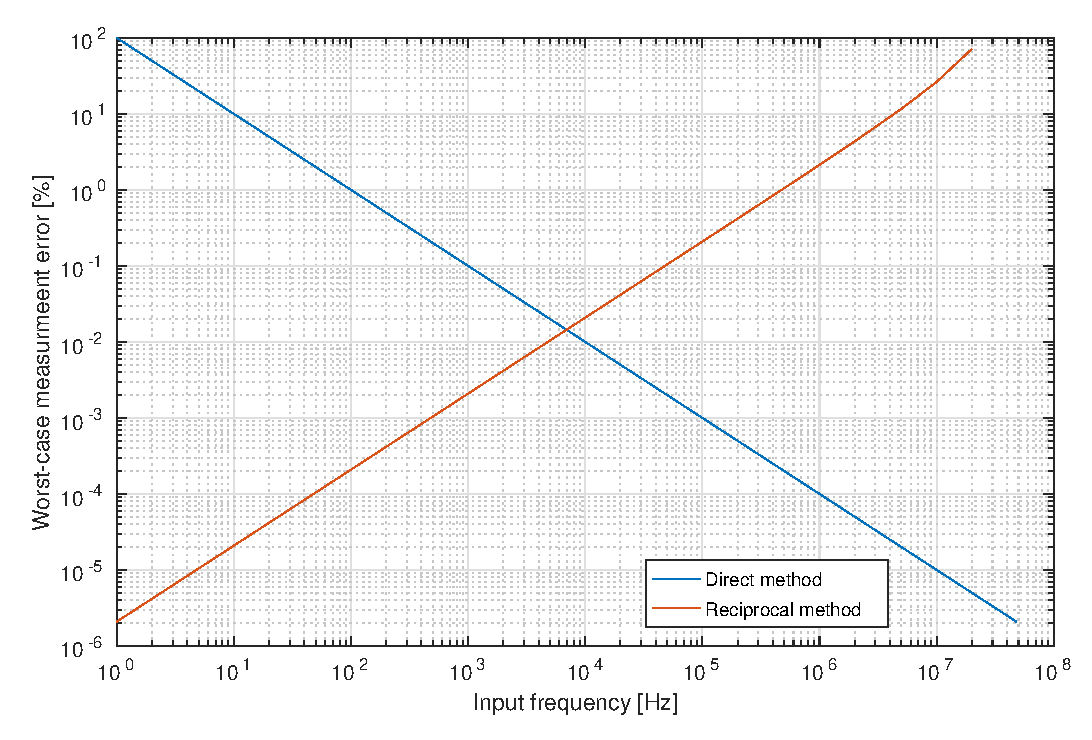
\includegraphics[width=.9\textwidth] {img/freqmethods.eps}
	\caption[Frequency measurement methods comparison]{\label{fig:freqmethods-graph}Worst-case error using the two frequency measurement methods with an ideal 48\,MHz timer clock. The crossing lies at 7\,kHz with an error of 0.015\,\%, or 1.05\,Hz.}
\end{figure}

Two basic methods to measure frequency exist, each with it's advantages and drawbacks:

\begin{itemize}
	\item The \textit{direct method} (fig. \ref{fig:fcap-direct-dia}) is based on the definition of frequency as a number of cycles $n$ in a fixed-length time window $\tau$ (usually 1\,s); the frequency is then calculated as $f=n/\tau$. 
	
	One timer generates the time window and its output gates the input of another, configured as a pulse counter. At the end of the measurement window an interrupt is generated and we can read the pulse count from the counter's register. 
	
	The direct method has a resolution of 1\,Hz with a sampling window of 1\,s (only a whole number of pulses can me counted). The resolution can be increased by using a longer time window, provided the measured signal is stable enough to make averaging possible without distorting the result.
	
	\item The \textit{indirect} or \textit{reciprocal method} (fig. \ref{fig:fcap-reci-dia}) measures one period $T$ as the time interval between two pulses and this is then converted to frequency as $f=1/T$. 
	
	This method needs only one timer/counter. Cycles of the system clock are counted for the duration of one period on the input pin (between two rising edges). If we additionally detect the falling edge in between, the counter's value gives us the duty cycle when related to the overall period length.
	
	Te reciprocal method's resolution depends on the counter's clock speed; if driven at 48\,MHz, the tick period is 20.83\,ns, which defines the granularity of our time measurement. It is common to measure several pulses and average the obtained values to further increase the precision. 
	
	We can easily achieve a sub-hertz resolution with this method, but its performance degrades at high frequencies where the time measurement precision becomes insufficient. The input frequency range can be extended using a hardware prescaller\footnote{\textit{Prescaller} is a divider implemented as part of the timer/counter peripheral block that can be optionally enabled and configured to a desired division factor.}, which is also applicable to the direct method, should the measurement of frequencies outside the counter's supported range be required. A duty cycle measurement available in this method can be used to read the output of sensors that use a pulse-width modulation.
\end{itemize}

Which method to use depends on the frequency we want to measure; the worst-case measurement errors of both methods, assuming an ideal 48\,MHz system clock, are plotted in figure \ref{fig:freqmethods-graph}. It can be seen that the reciprocal method leads in performance up to 7\,kHz where the direct method overtakes it. If a higher error is acceptable, the reciprocal method could be used also for higher frequencies to avoid a reconfiguration and to take advantage of its higher speed.

A good approach to a universal measurement, when we don't know the expected frequency beforehand, could be to first obtain an estimate using the direct method, and if the frequency is below the worst-case error crossing point (here 7\,kHz), to take a more precise measurement using the reciprocal method.

The system clock's frequency, which we use to measure pulse lengths and to gate the pulse counter, will be affected by tolerances of the used components, the layout of the PCB, temperature effects etc., causing measurement errors. A higher accuracy could be achieved using a temperature-compensated oscillator (TCO), or, in the direct method, by using the synchronization pulse provided by a GPS receiver to time the measurement interval.


\section{Analog Signal Acquisition} \label{sec:theory-adc}

\todo[inline]{Explain ADC operation and basic concepts / types}


\section{Waveform Generation} \label{sec:theory-dac}

A waveform generator is a useful tool in many experiments and measurements. A sine stimulus is the basis of a lock-in amplifier; it can be used to measure impedance; with a frequency sweep, we can obtain the frequency response of an analog filter, etc. We can, of course, generate other waveforms, such as a triangle, ramp, or rectangle wave.

The DAC peripheral can produce a DC level on the output pin based on a control word. When we periodically change its digital input, it produces an analog waveform. 

\subsection{Waveform Generation with DMA and a Timer} \label{sec:theory-dac-simple}

A straightforward implementation of the waveform generator is illustrated in figure \ref{fig:wavegen-naive}. This approach has its advantages: it's simple and works entirely in the background, with no interrupt handling required. It could even be implemented entirely in software, using a loop periodically updating the DAC values, of course such approach is less flexible and we would run into problems with asynchronous interrupts.

\begin{figure}
	\centering
	\includegraphics[scale=1] {img/wavegen-naive.pdf}
	\caption{\label{fig:wavegen-naive}A simple implementation of the waveform generator}
\end{figure}

The highest achievable output frequency largely depends on the size of our look-up table. For instance, assuming a timer frequency of 48\,MHz and a 8192-word table, holding one period of the waveform, the maximum frequency would be short of 6\,kHz, whereas if we shorten the table to just 1024 words, we can get almost 47\,kHz on the analog output. The downside of a shorter table is a lower resolution, which will appear as DC plateaus or steps when observed with an oscilloscope, producing harmonic components similar to those of a square wave.

A major disadvantage of this simple generation method is given by the limitations of the used timer, which defines the output frequency. Its output trigger fires when the internal counter reaches a pre-defined value, after which the counting register is reset. The counting speed is derived from the system clock frequency $f_\mathrm{c}$ using a prescaller $P$ and the set maximum value $N$. Only output frequencies that can be exactly expressed as $f=f_\mathrm{c}/(P\cdot N \cdot \mathrm{TableSize})$ can be accurately produced. Still, this simple and efficient method may be used where fine tuning is not required to take advantage of its fully asynchronous operation.

\subsection{Direct Digital Synthesis} \label{sec:theory-dac-dds}

There are situations where the simple waveform generation method is not sufficient, particularly when a fine tuning or on-line frequency and phase changes are required. Those are the strengths of a signal generation method called \textit{Direct Digital Synthesis} (DDS).

\begin{figure}[h]
	\centering
	\includegraphics[scale=1] {img/wavegen-dds.pdf}
	\caption{\label{fig:wavegen-dds}A block diagram of a direct digital synthesis waveform generator}
\end{figure}

A diagram of a possible DDS implementation in the STM32 firmware is shown in figure \ref{fig:wavegen-dds}. It is based on a \textit{numerically controlled oscillator} (NCO). NCO consists of a \textit{phase accumulator} register and a \textit{tuning word} which is periodically added to it at a constant rate in a timer interrupt handler. The value of the tuning word determines the output waveform frequency. The look-up table must have a power-of-two length so that it can be addressed by the \textit{n} most significant bits of the phase accumulator. An additional control word could be added to this address to implement a phase offset for applications like a phase-shift modulation.

The output frequency is calculated as \(f_\mathrm{out} = \dfrac{M\cdot f_\mathrm{c}}{2^n}\), where $M$ is the tuning word, $n$ is the bit length of the phase accumulator, and $f_c$ is the frequency of the phase-updating interrupt. The number of bits used to address the look-up table does not affect the output frequency; the table can be as large as the storage space allows. A tuning word value exceeding the lower part of the phase accumulator (including bits which directly enter the look-up address) will cause some values from the table to be skipped. A smaller tuning word, conversely, makes some values appear on the output more than once. This can be observed as steps or flat areas on the output. When the tuning word does not evenly divide $2^n$, that is, the modulo is non-zero, we can also observe jitter.

\subsubsection{DDS Implemented in Hardware}

DDS may be implemented in hardware, including the look-up table, often together with the DAC itself, which is then called a \textit{Complete DDS}. That is the case of e.g. AD9833 from Analog Devices. As the software implementation depends on a periodic interrupt, it's often advantageous to use a component like this when we need higher output frequencies where the use of an interrupt is not possible. GEX can control an external waveform generator like the AD9833 using an SPI port.

\todo[inline]{screenshots of a real demo, also reference to all-about-direct-digital-synthesis.pdf}


\section{Touch Sensing} \label{sec:theory-touch}

The used microcontroller, STM32F072, includes a touch sensing controller (TSC) peripheral block. It can be accessed from GEX as a demonstration of capacitive touch sensing, and could possibly be used for simple touch sensors as well, such as measuring the level of water in a tank.

\begin{figure}[h]
	\centering
	\includegraphics[width=0.5\textwidth] {img/disco-touch.jpg}
	\caption{\label{fig:disco-touch}The touch slider on a STM32F072 Discovery board}
\end{figure}

The TSC requires a specific topology with a sampling capacitor connected close to the microcontroller pin, which may not be possible on a universal GEX module; for this reason, the touch sensing feature is best demonstrated on the STM32F072 Discovery development kit, which includes a 4-segment touch slider shown in figure \ref{fig:disco-touch}.

The principle of capacitive touch sensing is well explained in the microcontroller's reference manual \todo{ref}. A key part of the TSC is a set of analog switches, which can be combined to form several different signal paths between the external pins, Vdd, GND, and an analog comparator. Two input pins are needed for every touch sensing channel: the sensing pad connects to one, the other is connected through a sampling capacitor  (47\,nF on the Discovery board) to GND. 

Capacitive sensing is a sequential process described in the following steps:

\begin{enumerate}
	\item The sensing capacitor is discharged by connecting its free end to GND.
	\item The sensing pad is connected to Vdd and, acting as a capacitor, charged to 3.3\,V. It stores a small amount of charge, depending on its capacitance---this is the variable property we are trying to measure.
	\item The free terminals of the two capacitors (the sensing pad and the sampling capacitor) are connected together and their voltages reach an equilibrium as a portion of the stored charge leaves the sensing pad and flows into the bigger capacitor.
	\item The steps (2) and (3) are repeated the sampling capacitor's voltage exceeds a fixed threshold (set to a half of the supply voltage). The number of cycles needed to charge the sampling capacitor corresponds to the capacitance of the sensing pad.
\end{enumerate}

\begin{figure}
	\centering
	\includegraphics[width=.9\textwidth] {img/tsc-wfm-bw.png} \\
	\vspace{5mm}
	\includegraphics[width=.9\textwidth] {img/tsc-wfm2-bw.png}
	\caption{\label{fig:tsc-wfm}A voltage waveform measured on the touch sensing pad. The bottom side of the envelope equals the sampling capacitor's voltage---this is the phase where both capacitors are connected. The detailed view (middle) shows the individual charging cycles. The bottom screenshot captures the entire waveform after the analog comparator was disabled.}
\end{figure}




\part{Implementation}

\chapter{Conceptual Overview} \label{sec:conceptual}

GEX is designed to be modular and easy to extend. The user-facing functionality is composed of independent software modules, called \textit{functional blocks} or \textit{units}, which can be configured by the user to fit their application needs. Units implement low-level logic to work with hardware peripherals of the microcontroller, and expose this functionality to the client application, running on the \gls{PC}, through a communication interface. A diagram showing the entire stack, from the user application down to hardware peripherals, is shown in \cref{fig:conceptual}.

\begin{figure}[h]
	\centering
	\includegraphics[scale=1]{img/conceptual.pdf}
	\caption[GEX conceptual overview]{\label{fig:conceptual}The ``GEX stack'', from a user application down to hardware}
\end{figure}

When we work with GEX, it is through units. The platform without units would be just an empty shell, the bare core framework; this underlying system will be described in \cref{sec:coreframework}. We will explore the individual units in \cref{sec:units_overview}, after going through the hardware realizations in \cref{sec:hwreal} and covering the communication protocol in \cref{sec:tinyframe}. 

\section{Physical User Interface}

The firmware can be flashed to a STM32 development board, or a custom \gls{PCB}. The particulars of those form factors will be discussed in \cref{sec:hwreal}.

\begin{figure}[h]
	\centering
	\includegraphics[scale=.95] {img/users-view.pdf}
	\caption{\label{fig:users_view_of_gex}Physical user interface of a GEX module}
\end{figure}

\noindent
All GEX hardware platforms have some common characteristics (\cref{fig:users_view_of_gex}):

\begin{itemize}	
	\item \textbf{Power \gls{LED}} -- a simple indication that the board is powered on
	\item \textbf{Status \gls{LED}} -- periodic flashing every 3\,s indicates correct operation, continuous light a software error\footnote{The microcontroller will then automatically restart within a few seconds due to a watchdog timeout.}; other light patterns may be shown as feedback to user actions or received commands
	\item \textbf{Reset button} -- resets the \gls{MCU}; this is particularly useful during firmware development as an alternative to re-connecting the \gls{USB} cable
	\item \textbf{Lock button} -- enables or disables access to configuration files through the virtual mass storage device
	\item \textbf{Boot button} -- when held during restart (that is, while the reset button is released), the \gls{DFU} mode~\cite{usbif-dfu} is activated and a new firmware image can be flashed over the \gls{USB} connection using \mono{dfu-util}~\cite{dfu-util} or other firmware update application
	\item \textbf{\gls{GPIO} header} -- a pin header exposing the \gls{MCU}'s \gls{GPIO} pins to be connected to external circuitry
	\item \textbf{Communication interface} -- a connection to the host \gls{PC}; multiple options may be available to choose from, a direct \gls{USB} connection being the primary and always available option
\end{itemize}

\section{GEX-PC Connection}

\Cref{fig:users_view_of_gex} shows three ways to connect the module to a \gls{PC}. Each communication interface has its advantages and drawbacks, and is suitable for different use-cases.

\begin{itemize}
	\item \textbf{Direct \gls{USB} connection}
		
		This is the primary and most straightforward connection method. We use the \gls{CDCACM} and \gls{MSC} \gls{USB} classes to have the module appear as a virtual COM port and a mass storage device, as described in \cref{sec:usb_classes}. This method is the fastest of the three and works out-of-the-box on Linux and MacOS. On MS Windows it may require the right software driver to be installed and assigned manually\footnote{The STM32 virtual COM port driver~\cite{stm-vcom} has been tested to work with GEX on MS Windows version 7 and 8, though it must be manually assigned to the device in the Device Manager. MS Windows 10 and later should support \gls{CDCACM} as a virtual COM port natively.}.
	
	\item \textbf{Hardware \gls{UART}}
	
		The hardware UART used as a communication interface is mapped to pins PA2 and PA3 to be compatible with the built-in \gls{USB}/\gls{UART} converter on STM32 Nucleo development boards. This interface is functionally identical to the \gls{CDCACM} connection, but the physical \gls{UART} is necessarily slower and does not implement flow control.
		
	\item \textbf{Wireless connection}
	
		A wireless connection is implemented using a radio module on the GEX board. To use it we need a counterpart, the \textit{wireless gateway}, which connects to the \gls{PC} via \gls{USB} and acts as a \gls{CDCACM} device.
	
\end{itemize}

The \gls{USB} connection is always enabled first on start-up. GEX waits its for enumeration by the host \gls{PC}. When not enumerated in a few seconds, it concludes that the interface is not active and tries other enabled options. The wireless module, connected through \gls{SPI}, can be detected by reading one of its registers that should have a known value. A \gls{UART} interface cannot be tested so reliably, thus it is always considered active\footnote{A detection of the UART connection would be possible by measuring the Rx pin voltage, which should idle at a high level (here 3.3\,V). This was not implemented in the initial firmware version.}.

\section{Controlling GEX}

GEX is a platform providing access to low-level hardware to high-level applications. However, this ``high level'' is relative. As was shown in \cref{fig:conceptual}, the ``GEX stack'' ends with a \textit{client library}, a software library used by the \textit{user application}.

The communication protocol (one level lower in the diagram) is robust and well defined, making it possible to implement alternative client libraries in other programming languages, or for yet-unsupported platforms. This protocol is explained in \cref{sec:tinyframe}. The client library implements the communication protocol and gives the user application access to GEX units via \textit{unit handles}. 

Any logic above the client library is in the hands of the user, which means that, to use GEX, they have to program a user application. Software libraries in languages C and Python are provided, and will be explained in \cref{sec:clientsw}. The Python library is easy to use even for beginner programmers, though we have to acknowledge that some users might not be familiar with programming at all. Making GEX more accessible to those users, e.g., through a graphical desktop application, is an appealing idea that is certainly worth pursuing in later work.

\section{Device Configuration}

The core framework and each of the units have a number of adjustable options determining their behavior. Those settings are internally stored in a binary form, but to make their adjustment comfortable for the user, they are mapped to text configuration files in the INI format.

\subsection{INI File Format}

INI files are, in our implementation, simple text files containing three basic syntax elements: comments, sections, and key-value entries. Sections group the key-value pairs into logical blocks, e.g., the configuration of individual units.

\begin{itemize}	
	\item \textbf{Comments} start with the hash symbol (\mono{\#}) and end at the end of line
	\item \textbf{Sections} are textual labels enclosed in square brackets (\mono{[UNITS]})
	\item \textbf{Key-value entries} are composed of a label, the equals sign, and its value; values may be text strings, decimal or hexadecimal numbers, lists of numbers separated by commas, or any other format appropriate for the particular key
\end{itemize}

\noindent
An example of the INI syntax is shown below.

\begin{inicode}
# comment
[section]
a = 123
b = 0xFF
port = A
pins = 1,2,3
\end{inicode}
	
\subsection{Configuration Files Structure}

The configuration is split into two files: \mono{UNITS.INI} and \mono{SYSTEM.INI}. The system configuration file has a simple structure and does not need much explanation beyond the comments already included in it; an example of its content is captured in \cref{lst:systemini}. The other file, as its name suggests, serves to configure GEX units.

\begin{listing}
	\begin{inicode}
		## SYSTEM.INI
		
		[SYSTEM]
		# Data link accessible as virtual comport (Y, N)
		expose-vcom=Y
		# Show comments in INI files (Y, N)
		ini-comments=Y
		# Enable debug UART-Tx on PA9 (Y, N)
		debug-uart=Y
		
		# Output core clock on PA8 (Y, N)
		mco-enable=N
		# Output clock prediv (1,2,...,128)
		mco-prediv=128
		
		# --- Allowed fallback communication ports ---
		
		# UART Tx:PA2, Rx:PA3
		com-uart=N
		com-uart-baud=115200
		
		# nRF24L01+ radio
		com-nrf=N
		# Radio channel (0-125)
		nrf-channel=76
		# Network prefix (hex, 4 bytes)
		nrf-network=12:00:09:4C
		# Node address (1-255)
		nrf-address=1
	\end{inicode}
	\caption{\label{lst:systemini}The \mono{SYSTEM.INI} configuration file}
\end{listing}

\begin{listing}
	\begin{inicode}
		## UNITS.INI
		
		[UNITS]
		# Create units by adding their names next to a type (e.g. DO=A,B),
		# remove the same way. Reload to update the unit sections below.
		
		# Digital output
		DO=led
		# Digital input with triggers
		DI=btn1,btn2
		# Neopixel RGB LED strip
		NPX=
		# I2C master
		I2C=i2c
		#...
		
		[I2C:i2c@1]
		# Peripheral number (I2Cx)
		#...
	\end{inicode}
	\caption{\label{lst:unitsini}Part of the \mono{UNITS.INI} configuration file}
\end{listing}

The units file, illustrated in \cref{lst:unitsini}, is more complex, and \textit{interactive}. The top part, a \mono{[UNITS]} section, lists all available unit types. A unit is created by writing its name (an arbitrary label composed of letters, numbers, and underscore) next to the desired type. Each unit is then configured in a separate section lower in the file; however, how does one know what keys are needed for which unit? This problem is solved by \textit{interactivity} of the file.

After adding a unit name next to its type, we save the file. The disk temporarily disappears from the device list as the file's content updates. When we reopen the file, a section for the new unit will be appended for us to configure as necessary. To delete a unit, it is sufficient to remove its name from the list at the top and let the file regenerate the same way; the unit's section will disappear.

It is not uncommon that the entered (or default) configuration is invalid and the unit cannot be enabled. The error is reported by inserting a comment into the INI file, at the top of the section of the failing unit. This error message disappears when the problem is corrected.

Once we are satisfied with the configuration, it may be stored to the module's permanent memory. This is done by pushing the Lock button again, which also deactivates the virtual storage device.

It may be interesting to know that the configuration files can also be read and modified through the communication interface. A simple configuration editor (\cref{fig:gexync}) was developed to demonstrate this feature. Besides applications like this, we can use the programmatic configuration access to change GEX settings automatically by the client application. The changes may be persisted by a command, but that is not required, which lets us use them temporarily without modifying the stored configuration.

\begin{figure}
	\centering
	\includegraphics[width=.8\textwidth] {img/gexync.png}
	\caption[Configuration file editor GUI]{\label{fig:gexync}Configuration file editor GUI built using the GEX client library and PyQt4}
\end{figure}




















\chapter{Application Structure}

GEX is designed to be modular and easy to extend. It's composed of a set of functional blocks, sometimes available in more than one instance, which can be configured by the user to fit their application needs. The firmware is built around a \textit{core framework} which provides services to the functional blocks, such as a settings storage, resource allocation, message delivery and periodic updates.

In this chapter, we will focus on the general function of the GEX module and will look at the services provided by the core framework. Individual functional blocks and the control API will be described in the following chapters.\todo{references}

\textit{A writing style note:} This and the following parts were written after implementing and evaluating the first hardware prototype and its firmware, therefore rather than describing the development process, it tends to talk about the completed solution and the decisions taken.

\section{User's View of GEX}

Before going into implementation details, we'll have a look at GEX from the outside, how an end user will see it. This should give the reader some context to better orient themselves in the following sections and chapters investigating the internal structure of the firmware and the communication protocol.

The GEX firmware can be flashed to a STM32 Nucleo or Discovery board or a custom PCB. It's equipped with a USB connector to connect to the host PC.  GEX loads its configuration from the non-volatile memory, configures its peripherals, sets up the function blocks and enables the selected communication interface(s). When USB is connected to the board, the PC enumerates it and either recognizes the communication interface as CDC/ACM (Virtual serial port), or leaves it without a software driver attached, to be accessed directly as raw USB endpoints. This can be configured. The user can now access the functional blocks using the client library and the serial protocol, as well as modify the configuration files.

The board is equipped with a button or a jumper labeled LOCK. When the button is pressed or the jumper removed, the Mass Storage USB interface is enabled. For the user this means a new disk will be detected by their PC's operating system that they can open in a file manager. This disk provides read and write access to configuration INI files and other files with useful information, like a list of supported features and available hardware resources. The user now edits a configuration file and saves it back to the disk. GEX processes the new content, tries to apply the changes and generates an updated version of the file that includes error messages if there was a problem. For the PC OS to recognize this change, the Mass Storage device momentarily reports that the media is unavailable to force the OS to reload it. This is a similar mechanism to what happens when a memory card is removed from a reader. Now the user must reload the file in their editor, inspect the updated content and perform any changes needed. The settings, when applied successfully, should now be available to test using the communication interface. When everything is to the user's satisfaction, the updated settings are committed to the device's non-volatile memory by pressing the LOCK button again, or replacing the jumper. 

For boards without a USB re-enumeration capability (notably with older microcontrollers like the STM32F103) that use a jumper, this must be removed before plugging the board to the host USB so that the Mass Storage is enabled immediately at start-up and a re-enumeration is not needed.

In the case when a wireless communication module is installed on the PCB and GEX is configured to use it, this will be used as a fallback when the USB peripheral does not receive an address (get enumerated) within a short time after start-up. The wireless link works in the same way as any other communication interface: it can be used to read and modify the configuration files and to access the functional blocks. To use it, the user needs to connect a wireless gateway module to their host PC and use the radio link instead of a USB cable. The gateway could support more than once GEX board at once.

Now that GEX is connected and configured, the user can start using it. This involves writing a program in C or Python that uses the GEX client library, using the Python library from MATLAB, or controlling GEX using a GUI front-end built on those libraries. The configuration can be stored in the module, but it's also possible to temporarily (or permanently) replace it using the communication API. This way the settings can be loaded automatically when the user's program starts.


\section{Functions of the Core Framework}

The core framework forms the skeleton of the firmware and usually doesn't need any changes when new user-facing features are added. It provides the following services:

\begin{itemize}
	\item Hardware resource allocation (\ref{sec:res-allocation})
	\item Settings storage and loading (\ref{sec:settings-storage})
	\item Functional block (\textit{units}) initialization (\ref{sec:units-function})
	\item The communication port with different back-ends: USB, UART, wireless (\ref{sec:com-ports})
	\item Message sending and delivery (\ref{sec:message_passing})
	\item Interrupt management and routing to functional blocks (\ref{sec:irq-routing})
	\item Virtual mass storage for configuration file editing
\end{itemize}

When the firmware needs to be ported to a different STM32 microcontroller, the core framework is relatively straightforward to adapt and the whole process can be accomplished in a few hours. The time consuming part is modifying the functional blocks to work correctly with the new device's hardware. 


\section{Resource Allocation} \label{sec:res-allocation}

\begin{figure}[h]
	\centering
	\includegraphics[scale=1] {img/resource-repository.pdf}
	\caption{\label{fig:resource-repository}An example allocation in the resource registry}
\end{figure}

The microcontroller provides a number of hardware resources that require exclusive access: GPIO pins, peripheral blocks (SPI, I2C, UART\textellipsis), DMA channels. If two units tried to control the same pin, the results would be unpredictable; similarly, with a multiple access to a serial port, the output would be a mix of the data streams and completely useless. 

To prevent a multiple access, the firmware includes a \textit{resource registry} (fig. \ref{fig:resource-repository}). Each individual resource is represented by a field in a resource table together with its owner's callsign. Initially all resources are free, except for those not available on the particular platform (i.e. a GPIO pin PD1 may be disabled if not present on the microcontroller's package). 

The resources used by the core framework are taken by a virtual unit \verb|SYSTEM| on start-up to prevent conflicts with the user's units. This is the case of the status LED, the LOCK button, USB pins, the communication UART, the pins and an SPI peripheral connecting the wireless module, pins used for the crystal oscillator, and the timer/counter which provides the system timebase.


\section{Settings Storage} \label{sec:settings-storage}

\begin{figure}[h]
	\centering
	\includegraphics[scale=1] {img/settings-storage.pdf}
	\caption{\label{fig:settings-storage}Structure of the settings subsystem}
\end{figure}

The system and unit settings are written, in a binary form, into designated pages of the microcontroller's Flash memory. The unit settings serialization and parsing is implemented by the respective unit drivers.

As the settings persist after a firmware update, it's important to maintain backwards compatibility. This is achieved by prefixing the unit's settings by a version number. When the settings are loaded by a new version of the firmware, it first checks the version and decides whether to use the old or new format. When the settings are next changed, the new format will be used.

The INI files, which can be edited through the communication API or using a text editor with the virtual mass storage, are parsed and generated on demand and are never stored in the Flash or RAM, other than in short temporary buffers. The INI parser processes the byte stream on-the-fly as it is received, and a similar method is used to build a INI file from the configured units and system settings.

\section{Functional Blocks} \label{sec:units-function}

GEX's user-facing functions, also called functional blocks or \textit{units}, are implemented in \textit{unit drivers}. Those are independent modules in the firmware that the user can enable and configure using the GEX configuration files. In principle, there can be multiple instances of each unit type. However, we are limited by hardware constraints: there may be only one ADC peripheral, two SPI ports and so on. The mutually exclusive assignment of resources to units is handled by the \textit{resource registry} (\ref{sec:res-allocation}).

Each unit is defined by a section in the configuration file \verb|UNITS.INI|. It is given a name and a \textit{callsign}, which is a number that serves as an address for message delivery. A unit is internally represented by a data object with the following structure:

\begin{itemize}
	\item Name
	\item Callsign
	\item Configuration parameters loaded from the unit settings
	\item State variables updated at run-time by user commands or internal functions
	\item A reference to the unit driver
\end{itemize}

The unit driver handles commands sent from the host PC, initializes and de-initializes the unit based on its settings, and implements other aspects of the unit's function, such as periodic updates and interrupt handling. Unit drivers may expose public API functions to make it possible to control the unit from a different driver, allowing the creation of "macro units".

\section{Source Code Layout}

\begin{wrapfigure}[20]{r}{0.4\textwidth}
	\scriptsize\vspace{-3em}
	\begin{verbatim}
├── build
│   ├── firmware.bin
│   └── firmware.dfu
├── Drivers
│   ├── CMSIS
│   │   └── Device / ST / STM32F0xx
│   └── STM32F0xx_HAL_Driver
├── Middlewares / Third_Party / FreeRTOS
├── Src
│   └── main.c
├── User
│   ├── USB / STM32_USB_Device_Library
│   │   ├── Class
│   │   │   ├── CDC
│   │   │   ├── MSC
│   │   │   └── MSC_CDC
│   │   └── Core
│   ├── platform
│   │   ├── plat_compat.h
│   │   └── platform.c
│   ├── units
│   │   ├── adc
│   │   ├── digital_out
│   │   ...
│   ├── FreeRTOSConfig.h
│   └── gex.mk
└── Makefile	
	\end{verbatim}
	\vspace{-1em}
	\cprotect\caption{\label{fig:repo-structure} The general structure of the source code repository}
\end{wrapfigure}

Looking at the source code repository (fig. \ref{fig:repo-structure}), at the root we'll find device specific driver libraries and files provided by ST Microelectronics, the FreeRTOS middleware, and a folder called \verb|User| containing the GEX application code. This division is useful when porting the firmware to a different microcontroller, as the GEX folder is mostly platform-independent and can be simply copied (of course, adjustments are needed to accompany different hardware peripheral versions etc.). The GEX core framework consists of everything in the \verb|User| folder, excluding the \verb|units| directory in which the individual units are implemented. Each unit driver must be registered in the file \verb|platform.c| to be available for the user to select. The file \verb|plat_compat.c| includes platform-specific headers and defines e.g. which pin to use for a status LED or the LOCK button.

The USB Device library, which had to be modified to support a composite class, is stored inside the \verb|User| folder too, as it is compatible with all STM32 microcontrollers that support USB.


\section{Communication Ports} \label{sec:com-ports}

The firmware supports three different communication ports: hardware UART, USB (virtual serial port), and a wireless connection. Each interface is configured and accessed in a different way, but for the rest of the firmware (and for the PC-side application) they all appear as a full duplex serial port. To use interfaces other than USB, the user must configure those in the system settings (a file \verb|SYSTEM.INI| on the configuration disk).

At start-up, the firmware enables the USB peripheral, configures the device library and waits for enumeration by the host PC. When not enumerated, it concludes the USB cable is not connected, and tries some other interface. The UART interface can't be tested as reliably, but it's possible to measure the voltage on the Rx pin. When idle, a UART Rx line should be high (here 3.3\,V). The wireless module, when connected using SPI, can be detected by reading a register with a known value and comparing those.

\subsection{USB Connection}

GEX uses vid:pid \verb|1209:4c60| and the wireless gateway \verb|1209:4c61|. The USB interface uses the CDC/ACM USB class (\ref{sec:cdc-acm}) and consists of two bulk endpoints with a payload size of up to 64 bytes.

\subsection{Communication UART}

The parameters of the communication UART (such as the baud rate) are defined in \verb|SYSTEM.INI|. It's mapped to pins PA2 and PA3; this is useful with STM32 Nucleo boards that don't include a User USB connector, but provide a USB-serial bridge using the on-board ST-Link programmer, connected to those pins. 

This is identical to the USB connection from the PC application's side, except a physical UART is necessarily slower and does not natively support flow control. The use of the Xon and Xoff software flow control is not practical with binary messages that could include those bytes by accident, and the ST-Link USB-serial adapter does not implement hadware flow control.

\subsection{Wireless Connection}

The wireless connection uses an on-board communication module and a separate device, a wireless gateway, that connects to the PC. The wireless gateway is interfaced differently from the GEX board itself, but it also shows as a virtual serial port on the host PC. This is required to allow communicating with the gateway itself through the CDC/ACM interface in addition to addressing the end devices.

This interface will be explained in more detail in chapter \ref{sec:wireless}.

\section{Message Passing} \label{sec:message_passing}

One of the key functions of the core framework is to deliver messages from the host PC to the right units. This functionality resides above the framing protocol, which will be described in chapter \ref{sec:tinyframe}.

A message that is not a response in a multi-part session (this is handled by the framing library) is identified by its Type field. Two main groups of messages exist: \textit{system messages} and \textit{unit messages}. System messages can access the INI files, query a list of the available units, restart the module etc. Unit messages are addressed to a particular unit by their callsign (see \ref{sec:units-function}), and their payload format is defined by the unit driver. The framework reads the message type, then the callsign byte, and tries to find a matching unit in the unit list. If no unit with the callsign is found, an error response is sent back, otherwise the unit driver is given the message to handle it as required.

The framework provides one more messaging service to the units: event reporting. An asynchronous event, such as an external interrupt, an ADC trigger or an UART data reception needs to be reported to the host. This message is annotated by the unit callsign so the user application knows it's origin.


\section{Interrupt Routing} \label{sec:irq-routing}

Interrupts are an important part of almost any embedded application. They provide a way to rapidly react to asynchronous external or internal events, temporarily leaving the main program, jumping to an interrupt handler routine, and then returning back after the event is handled. Interrupts are also the way FreeRTOS implements multitasking without a multi-core processor.

In the Cortex-M0-based STM32F072, used in the initial GEX prototypes, the interrupt handlers table, defining which routine is called for which interrupt, is stored in the program memory and can't be changed at run-time. This is a complication for the modular structure of GEX where different unit drivers may use the same peripheral, and we would want to dynamically assign the interrupt handlers based on the active configuration. Let's have a look at an interrupt handler, in this case handling four different DMA channels, as is common in STM32 microcontrollers:

\begin{minted}{c}
void DMA1_Channel4_5_6_7_IRQHandler(void)
{
    if (LL_DMA_IsActiveFlag_GI4(DMA1)) { /* handle DMA1 channel 4 */ }
    if (LL_DMA_IsActiveFlag_GI5(DMA1)) { /* handle DMA1 channel 5 */ }
    if (LL_DMA_IsActiveFlag_GI6(DMA1)) { /* handle DMA1 channel 6 */ }
    if (LL_DMA_IsActiveFlag_GI7(DMA1)) { /* handle DMA1 channel 7 */ }
}
\end{minted}

It is evident that multiple units might need to use the same interrupt handler, even at the same time, since each DMA channel is configured, and works, independently. GEX implements a redirection scheme to accomplish such interrupt sharing: All interrupt handlers are defined in one place, accompanied by a table of function pointers. When a unit driver wants to register an interrupt handler, it stores a pointer to it in this redirection table. Then, once an interrupt is invoked, the common handler checks the corresponding entry in the table and calls the referenced routine, if any. Conversely, when a unit driver deinitializes a unit, it removes all interrupt handlers it used, freeing the redirection table slots for other use.












\chapter{Working with the GEX Source Code}

\begin{wrapfigure}[20]{r}{0.4\textwidth}
	\scriptsize\vspace{-3em}
	\begin{verbatim}
├── build
│   ├── firmware.bin
│   └── firmware.dfu
├── Drivers
│   ├── CMSIS
│   │   └── Device / ST / STM32F0xx
│   └── STM32F0xx_HAL_Driver
├── Middlewares / Third_Party / FreeRTOS
├── Src
│   └── main.c
├── User
│   ├── USB / STM32_USB_Device_Library
│   │   ├── Class
│   │   │   ├── CDC
│   │   │   ├── MSC
│   │   │   └── MSC_CDC
│   │   └── Core
│   ├── platform
│   │   ├── plat_compat.h
│   │   └── platform.c
│   ├── units
│   │   ├── adc
│   │   ├── digital_out
│   │   ...
│   ├── freertos.c
│   ├── FreeRTOSConfig.h
│   └── gex.mk
└── Makefile
	\end{verbatim}
	\vspace{-1em}
	\caption{\label{fig:repo_structure} General structure of the source code repository}
\end{wrapfigure}

Understanding the GEX source code layout is important before attempting to implement any changes or to port it to a different microcontroller type. The directory layout is shown in \cref{fig:repo_structure}. 

The GEX core framework resides in the User folder, and units are defined in User/units. Each unit driver must be registered in the file \verb|platform.c|. The header file \verb|plat_compat.h| defines platform-specific constants and macros, defining parameters such as pin assignments or the clock speed. The User folder is actually a Git submodule called ``gex-core'' and is kept as a separate project; platform-specific customizations are managed using compile flags passed from the Makefile.

\section{Porting to a New Platform}

When porting GEX to a new platform, the basis of the project can be generated by the STM32CubeMX code generator \cite{cubemx}, using the Makefile output preset. We have to enable FreeRTOS, select a USB class (the choice does not matter, e.g., \gls{CDCACM} can be used), and configure the system clock. 

The configuration dialog gives a choice between the LL (Low Level) and HAL driver libraries; the HAL library uses a lot of program memory and often contains software bugs, while the LL library is leaner but harder to use. The LL library was used in the STM32F072 port for its smaller size.

Some files generated by STM32CubeMX were moved into the User folder (e.g., the FreeRTOS configuration and initialization, or the system time base generation), as they are mostly platform-independent. The modified \gls{USB} Device library was copied here as well, as it had to be modified to support the definition of a composite class with custom descriptors.

The rest of the porting process, after generating the base project, can be summarized in the following bullet points. These are written as a checklist for the developer working on a new port; an existing, functional port may be consulted as a reference during the porting process.

\begin{itemize}	
	\item Initialize the project folder as a Git repository.
	
	\item Add the ``gex-core'' Git submodule as the \verb|User| folder, and create a Git branch in it for the new platform.
	
	\item Fix the Makefile generated by STM32CubeMX; it usually contains duplicate entries in the file lists and other errors. Ensure the build (``\verb|make|'' invocation in the terminal) succeeds before making any other changes.
	
	\item Delete the USB Device library from the \verb|Middlewares/ST| folder; GEX uses the modified version included in \verb|User/USB|.
	
	\item Move the \gls{GPIO}, FreeRTOS, USB, and other peripheral initialization from \verb|Src| and \verb|Inc| aside for later reference; the code in those folders should only configure the system clock, call the GEX initialization function ``\verb|GEX_PreInit()|'', and start FreeRTOS with ``\verb|MX_FREERTOS_Init()|'' and ``\verb|osKernelStart()|''.
	
	\item Add ``\verb|include User/gex.mk|'' and ``\verb|GEX_PLAT=MYPLATFORM|'' at the top the Makefile, with the desired platform name in place of ``\verb|MYPLATFORM|''; the name must be a valid C identifier.
	
	\item Add ``\verb|GEX_CFLAGS|'', ``\verb|GEX_SOURCES|'', ``\verb|GEX_INCLUDES|'', ``\verb|GEX_CDEFS|'' into the appropriate file lists in the Makefile; those variables are exported from \verb|User/gex.m| and contain lists of GEX source files and compiler flags.
	
	Use ``\verb|$(foreach x,$(GEX_SRC_DIR),$(wildcard $(x)/*.c))|'' to include all source files from ``\verb|GEX_SRC_DIR|'' in the ``\verb|C_SOURCES|'' list.
	
	\item Remove all definitions of ``\verb|Error_Handler()|'', ``\verb|FULL_ASSERT|'' and ``\verb|assert_param()|'' from the files left inside \verb|Inc| and \verb|Src|, and add ``\verb|#include "stm32_assert.h"|'' to \verb|Src/main.h|. GEX uses the functions declared in \verb|User/stm32_assert.h| for assertions.
	
	\item Update \verb|User/FreeRTOSConfig.h| and \verb|User/platform/plat_compat.h| for the new platform. Preprocessor directives like ``\verb|#ifdef|'' are used to define configuration applicable only to one platform, without affecting others.
	
	\item Update \verb|User/platform/platform.c| to register the initially supported units; a good choice is the DO (Digital Output) unit that is straightforward to update and can be used to verify the platform's functionality.
	
	Define a flag like ``\verb|UNIT_DO=1|'' at the top of the Makefile for each registered unit. \verb|User/gex.m| may be used as a reference for the expected variable names. This is used to conditionally enable or disable the inclusion of the particular unit's source files in the compilation.
	
	\item Update the USB functions in the \verb|User/USB| folder according to the ones previously generated by STM32CubeMX. The USB Device library uses these as an interface to the different \gls{USB} peripheral versions.
	
	\item Update other platform-dependent code (such as the debug \gls{UART} configuration). The compiler should warn about those occurrences when trying to build the project.	
	
	\item Try to build the project by running ``\verb|make|'' in the terminal.
\end{itemize}

After the firmware successfully compiles, we can flash it to the \gls{MCU} using ST-Link by running ``\verb|make flash|'', or through the \gls{DFU} interface with ``\verb|make dfu|''. 

The first thing to verify after flashing the firmware is that the debug \gls{UART}'s configuration is correct and we can see the log output, which should be available on pin PA9 at 115200\,baud. Thanks to a generous usage of assertions, most errors should produce helpful log messages in the log. We can then proceed to experiment with the device, testing the features described in \cref{sec:conceptual} while observing the debug log for any anomalies.

\chapter{Communication Protocol} \label{sec:tinyframe}

GEX can be controlled through a hardware \gls{UART}, the \gls{USB} or over a wireless link. To minimize the firmware complexity, all the three connection methods are handled by the same protocol stack and are functionally interchangeable.

The communication is organized in transactions. A transaction consists of one or more messages going in either direction. Messages can be stand-alone, or chained with a response or a follow-up message using the transaction ID. Both peers, GEX and the client application running on the host PC, are equal in the communication: either side can independently initiate a transaction at any time.

GEX uses a framing library \textit{TinyFrame}, developed likewise by the author but kept as a separate project for easier re-use in different applications. The library implements frame building and parsing, checksum calculation and a system of message listeners.

\section{Frame Structure}

Message frames have the following structure (all little-endian):

\begin{boxedpayload}[``TinyFrame'' frame structure, as used in GEX]
	\cfield{u8} start-of-frame marker (0x01)
	\cfield{u16} frame ID
	\cfield{u16} payload length
	\cfield{u8} frame type
	\cfield{u8} header checksum	
	\cfield{u8[]} payload
	\cfield{u8} payload checksum (omitted for empty payloads)
\end{boxedpayload}

\iffalse
\begin{table}[h]
	\centering
	%\hspace{-1.5em}
	\begin{tabular}{rccccccc}
		\toprule
		\multicolumn{1}{c|}{} &
		\multicolumn{5}{c}{Header}&
		\multicolumn{2}{|c}{Body} \\
		\midrule
		%
		\textit{Field} &
			\textbf{SOF} &
			\textbf{Frame ID} &
			\makecell{ \Gape{\textbf{Payload}} \\ \Gape{\textbf{Length}} } &
			\makecell{ \textbf{Frame} \\ \textbf{type} } &
			\makecell{ \textbf{Header} \\ \textbf{checksum} } &
			\textbf{Payload} &
			\makecell{ \textbf{Payload} \\ \textbf{checksum} } \\
		%
		\midrule
		\textit{Bytes} &
			 1  &
			 2  &
			 2  &
			 1  &
			 1  &
			 ... &
			 1 \\
		%
		\bottomrule
	\end{tabular}
\end{table}
\fi

\textit{Frame ID}, which could be better described as \textit{Transaction ID}, uniquely identifies each transaction. The most significant bit is set to a different value in each peer to avoid ID conflicts, and the rest of the ID field is incremented with each initiated transaction.

\section{Message Listeners}

After sending a message that should receive a response, the peer registers an \textit{ID listener} with the ID of the sent message. A response reuses the original frame ID and when it is received, this listener is called to process it. ID listeners can also be used to receive multi-part messages re-using the original ID.

\textit{Frame type} describes the payload and does not have any prescribed format; the values are defined by application (here, GEX). A \textit{type listener} may be registered to handle all incoming messages with a given frame type. It works in a similar way to an ID listener and has a lower priority.

Each message can be handled by only one listener, unless it explicitly requests the message to be passed on to a lower priority one. Messages unhandled by any listener are given to a default listener, which can e.g. write an error to a debug log.

\section{Designated Frame Types}

The following table lists all frame types used by GEX. It is divided into four logical sections: General, Bulk Read/Write, Unit Access, and Settings.

\begin{table*}[h]
	\centering
	\begin{tabular}{clll}
		\toprule
		\textbf{Frame type} & \textbf{Function} & \textbf{Note} \\
		\midrule
		0x00 & Success & \textit{Payload depends on context} \\
		0x01 & Ping & \textit{GEX responds with Success and its version string} \\
		0x02 & Error & \textit{Payload contains the error message} \\
		\midrule
		0x03 & Bulk Read Offer & \textit{An offer of data to read using }0x04 \\
		0x04 & Bulk Read Poll & \textit{Requesting to read a block of data} \\
		0x05 & Bulk Write Offer & \textit{An offer to receive a bulk write transaction} \\
		0x06 & Bulk Data & \textit{Used for both reading and writing} \\
		0x07 & Bulk End & \textit{Marks the last ``Bulk Data'' frame} \\
		0x08 & Bulk Abort & \textit{} \\
		\midrule
		0x10 & Unit Request & \textit{Request to a unit} \\
		0x11 & Unit Report & \textit{Spontaneous event generated by a unit} \\
		\midrule
		0x20 & List Units & \textit{Read a list of all instantiated units} \\
		0x21 & INI Read & \textit{Request a bulk read transaction of an INI file} \\
		0x22 & INI Write & \textit{Request a bulk write transaction of an INI file} \\
		0x23 & Persist Config & \textit{Write updated configuration to Flash} \\
		\bottomrule
	\end{tabular}
\end{table*}


\section{Bulk Read and Write Transactions} \label{sec:tf-bulk-rw}

The bulk read and write transactions are generic, multi-message exchanges which are used to transfer the INI configuration files. They could additionally be used by some future unit requiring to transfer a large amount of data (e.g. to read image data from a camera).

The reason for splitting a long file into multiple messages, rather than sending it all in one, lies in the hardware limitations of the platform, specifically its small amount of \gls{RAM} (the STM32F072 has only 16\,kB). A message cannot be processed until its payload checksum is received and verified; however, the configuration file can have several kilobytes, owning to the numerous explanatory comments, which would require a prohibitively large data buffer. The chunked transaction could, additionally, be extended to support message re-transmission on timeout without sending the entire file again.

A read or write transaction can be aborted by a frame 0x08 (Bulk Abort) at any time, though aborting a write transaction may leave the configuration in a corrupted state. As hinted in the introduction of this chapter, a transaction is defined by sharing a common frame ID. Thus, all frames in a bulk transaction must have the same ID, otherwise the ID listeners won't be called for the subsequent messages, and the transaction will time out.

Figure \ref{fig:bulk-rw} shows a diagram of the bulk read and write data flow.

\begin{figure}
	\centering
	\includegraphics[scale=1.5]{img/bulk-read-write.pdf}
	\caption{\label{fig:bulk-rw}A diagram of the bulk read and write transaction.}
\end{figure}

\subsection{Bulk Read}

To read an INI file, we first send a frame 0x21 (INI Read), specifying the target file in the payload:

\begin{boxedpayload}[INI Read frame structure]
	\cfield{u8} which file to write
		\begin{pldlist}
			\item 0 \dots UNITS.INI
			\item 1 \dots SYSTEM.INI
		\end{pldlist}
\end{boxedpayload}

What follows is a standard bulk read transaction with the requested file.
GEX offers the file for reading with a frame 0x03 (Bulk Read Offer):

\begin{boxedpayload}[Bulk Read frame structure]
	\cfield{u32} full size of the file in bytes
	\cfield{u32} largest chunk that can be read at once
\end{boxedpayload}

Now we can proceed to read the file using 0x04 (Bulk Read Poll), which is always responded to with 0x06 (Bulk Data), or 0x07 (Bulk End) if this was the last frame. Data frames have only the useful data as their payload.

The 0x04 (Bulk Read Poll) payload specifies how many bytes we want to read:

\begin{boxedpayload}[Bulk Read Poll frame structure]
	\cfield{u32} how many bytes to read (at most)
\end{boxedpayload}

\subsection{Bulk Write}

To overwrite an INI file, we first send a frame 0x22 (INI Write) with the file size as its payload. The name of the file is irrelevant, as it's detected automatically by inspecting the content.

\begin{boxedpayload}[INI Write frame structure]
	\cfield{u32} size of the written file, in bytes
\end{boxedpayload}

The write request is confirmed by a frame 0x05 (Bulk Write Offer) sent back:

\begin{boxedpayload}[Bulk Write Offer frame structure]
	\cfield{u32} total bytes to write (here copied from the request frame)
	\cfield{u32} how many bytes may be written per message
\end{boxedpayload}

We can now send the file as a series of frames 0x06 (Bulk Data), or 0x07 (Bulk End) in the last frame, with chunks of the data as their payload. Each frame is confirmed by 0x00 (Success).

\begin{boxedpayload}[Bulk Data or Bulk End frame structure]
	\cfield{u8[]} a chunk of the written file
\end{boxedpayload}

\subsection{Persisting the Changed Configuration to Flash}

The written INI file is immediately parsed and the settings are applied. However, those changes are not persistent: they exist only in RAM and will be lost when the module restarts. To save the current state to Flash, issue a frame 0x23 (Persist Config). This has the same effect as pressing the LOCK button (or replacing the LOCK jumper) when the INI files are edited using the virtual mass storage.

It should be noted that after flashing a firmware, the Flash control registers may remain in an unexpected state and the module must first be manually restarted before attempting to persist settings. Otherwise an assertion will fail and the module is restarted by a watchdog, losing the temporary changes.

% TODO there must be a workaround, and then this paragraph can be removed.


\section{Reading a List of Units}

The frame 0x20 (List Units) requests a list of all available units in the GEX module. The list includes all units' callsigns, names and types. The response payload has the following format (in pseudocode):

\begin{boxedpayload}[List Units response structure (frame type Success)]
	\cfield{u8} the number of available units
	\item For each unit:
		\begin{pldlist}
			\cfield{u8} unit callsign
			\cfield{char[]} unit name (zero-terminated string)
			\cfield{char[]} unit type (zero-terminated string)
		\end{pldlist}
\end{boxedpayload}


\section{Unit Requests and Reports} \label{sec:unit_requests_reports}

Frame types 0x10 (Unit Request) and 0x11 (Unit Report) are dedicated to messages sent to and by unit instances. Each has a fixed header (\textit{inside the payload}) followed by unit-specific data.

\subsection{Unit Requests}

Unit requests deliver a message from the host to a unit instance. Unit drivers implements different commands, each with its own payload structure. The frame 0x10 (Unit Request) has the following structure:

\begin{boxedpayload}[Unit Request frame structure]
	\cfield{u8} unit callsign
	\cfield{u8} command number, handled by the unit driver
	\cfield{u8[]} command payload, handled by the unit driver; its size and content depend on the unit driver and the particular command number
\end{boxedpayload}

The most significant bit of the command byte (0x80) has a special meaning: when set, the message delivering routine responds with 0x00 (Success) after the command completes, unless an error occurred. That is used to get a confirmation that the message was delivered and the module operates correctly (as opposed to e.g. a lock-up resulting in a watchdog reset). Requests which normally generate a response (e.g. reading a value from the unit) should not be sent with this bit set. As a result of this special treatment of the highest bit, there can be only 127 different commands per unit.

\subsection{Unit Reports}

Several unit types can produce asynchronous events, such as reporting a pin change or a triggering condition. The event is timestamped and sent with a frame type 0x11 (Unit Report):

\begin{boxedpayload}[Unit Report (event) frame structure]
	\cfield{u8} unit callsign
	\cfield{u8} report type, defined by the unit driver
	\cfield{u64} event time (microseconds since power-on)
	\cfield{u8[]} report payload; its size and content depend on the unit driver and the particular report type
\end{boxedpayload}


















\chapter{Wireless Interface} \label{sec:wireless}

Four methods of a wireless connection have been considered: Bluetooth (e.g. with CC2541), WiFi with ESP8266, a 868\,MHz long range link with SX1276, and a 2.4\,GHz link with nRF24L01+. Bluetooth was dismissed early for its complexity, and ESP8266 for its high consumption in continuous reception mode, although both solutions might be viable for certain applications and with more development time. 

The Semtech SX1276 and Nordic Semiconductor nRF24L01+ transceivers have both been tested using the first GEX prototype, confirming its usefulness as a hardware development tool, and it's been confirmed they could fulfill the requirements of the application.

\begin{figure}[h]
	\centering
	\includegraphics[width=.7\textwidth]{img/nrf-testing.jpg}
	\caption{Test setup with a GEX prototype controlling two nRF24L01+ modules}
\end{figure}

\section{Modulations Overview}

A brief overview of the different signal modulation techniques is presented here to aid the reader with understanding of table \ref{fig:nrf-sx-comparison} and the rest of the chapter.

\subsection{On-Off Keying (OOK)}

In \gls{OOK}, the carrier generator is switched on and off to transmit ones and zeros. 

\subsection{Frequency Shift Keying (FSK)}

\Gls{FSK} uses a change of the carrier frequency to transmit data. The simplest form of \gls{FSK} is \gls{BFSK}, which uses a pair of alternating frequencies to transmit ones and zeros.

\subsection{Gaussian Frequency Shift Keying (GFSK)}

\Gls{GFSK} is an improvement over basic \gls{FSK} which does not switch between the different frequencies instantaneously, but uses a Gaussian filter to make the changes less abrupt, which reduces the side-band interference otherwise generated by the sharp edges. This scheme can be imagined as sending the binary waveform through a Gaussian filter and then modulating a \gls{VCO} with its output, rather than changing the \gls{VCO}'s control voltage discretely. \Gls{GFSK} is used in the Bluetooth standard.

\subsection{Minimum-Shift Keying (MSK)}

\Gls{MSK} is another \gls{FSK}-based modulation scheme. In \gls{MSK}, the frequencies representing different symbols are chosen such that there are no sharp changes in the phase of the output waveform, the modulation is \textit{phase-coherent}. This is another way to reduce side-band interference.

\subsection{Gaussian Minimum-Shift Keying (GMSK)}

\Gls{GMSK} is a variant of \gls{MSK} which uses a gaussian filter to shape the digital signal before sending it to the oscillator. The principle is similar to \gls{GFSK}, and it is yet another way to further reduce side-band interference and increase spectral efficiency. GMSK is used in the \gls{GSM}.

\subsection{LoRa Modulation}

LoRa is a patented proprietary modulation developed by Semtech. It uses a direct sequence frequency hopping spread spectrum modulation and can achieve very long range transmission (over 10\,km is not uncommon). LoRa is available only with transceiver \glspl{IC} produced by Semtech and for this reason it is rather expensive.

\section{Comparing SX1276 vs. nRF24L01+}

The two transceivers are compared in table \ref{fig:nrf-sx-comparison}. It's apparent that each has its strengths and weaknesses.

\begin{table}[h]
	\centering
	\begin{tabulary}{\textwidth}{lLL}
		\toprule
		\textbf{Parameter} & \textbf{SX1276} & \textbf{nRF24L01+} \\
		\midrule
		\textbf{Connection} & SPI (4 pins) + up to 6 IRQ & SPI (4 pins), CE, IRQ \\
		\textbf{Frequency band} & 868\,MHz or 433\,MHz & 2.4\,GHz \\
		\textbf{Data rate} & up to 300\,kbps & 250--2000\,kbps \\
		\textbf{Modulation} & (G)FSK, (G)MSK, OOK, LoRa & GFSK \\
		%		\textbf{Bandwidth} & 7--500\,kHz per channel & 0.7--2\,MHz per channel \\
		\textbf{Range (est.)} & 2\,km to 20\,km LOS & up to 1\,km LOS \\
		\textbf{Consumption Rx} & 10.8--12\,mA & 12.6--13.5\,mA \\
		\textbf{Consumption Tx} & 20--120\,mA & 7--11.3\,mA \\
		\textbf{Idle power (max)} & 1\,$\mu$A sleep, 2\,mA stand-by & 0.9\,$\mu$A sleep, 320\,$\mu$A stand-by \\
		\textbf{Max packet size} & 300 bytes & 32 bytes \\
		\textbf{Reset} & NRESET pin & Vdd disconnect \\
		\textbf{Extra} & LoRa FHSS, packet engine & ShockBurst protocol engine \\
		\textbf{Price} & \$7.3 & \$1.6 \\
		\bottomrule
	\end{tabulary}
	\caption[Comparison of the SX1276 and nRF24L01+ wireless transceivers]{\label{fig:nrf-sx-comparison}Comparison of the SX1276 and nRF24L01+ wireless transceivers (price from DigiKey @ 10 pieces, May 6th 2018)}
\end{table}

SX1276 supports additional modulation modes, including a proprietary LoRa scheme with a frequency-hopping spread spectrum modulation that can be received at a distance up to 20\,km in ideal conditions. The long-range capability is reflected in a higher consumption during transmission. However, its consumption in receiver mode is slightly lower than that of the nRF24L01+.

nRF24L01+ provides higher data rates at short distances. Its power consumption is comparable or lower than that of the SX1276. It lacks a dedicated reset pin, but that can be easily worked around using an external transistor to momentarily disconnect its Vdd pin.

Both devices implement some form of a packet engine with error checking; that of the nRF24L01+, called ShockBurst, is more advanced as it implements acknowledgment responses and automatic re-transmission, leading to a potentially more robust communication without an additional overhead on the side of the microcontroller. 


\section{Integration of the nRF24L01+ into GEX}

The nRF24L01+ was selected to be integrated into GEX thanks to its inclusion of the ShockBurst engine, higher possible data rates and significantly lower price. The SX1276, nonetheless, remains an interesting option that could be used as an alternative in the future, should the need for a long range communication arise.

A separate device, the \textit{GEX wireless gateway}, was developed to provide the PC connection to a nRF24L01+ module. It is based on the STM32F103 microcontroller in its smallest package (LQFP48), selected for it's low cost and good availability.

\subsection{The Wireless Gateway Protocol}

\begin{wrapfigure}[17]{r}{0.38\textwidth}
	\vspace{-1em}
	\centering
	\includegraphics[scale=0.9]{img/rf-gw.pdf}
	\caption{A block diagram of the wireless connection}
\end{wrapfigure}

The gateway presents itself to the host as a \gls{CDCACM} device, much like the GEX modules themselves (here called \textit{nodes}) when connected over \gls{USB}. It implements a simple protocol which encapsulates the binary data sent to or from a connected node. The wrapped GEX protocol (chapter \ref{sec:tinyframe}) remains unchanged.

The gateway has a 4-byte network ID, a number derived from the microcontroller's unique ID. The network ID must be entered into all nodes that wish to communicate with it. Additionally, each module must be assigned a unique 1-byte number, which, together with the four network ID bytes, uniquely identifies the node. The gateway can connect to up to 6 nodes at once.

All messages sent to or from the gateway are a multiple of 64 bytes long, padded with zeros if shorter. The message starts with a control byte, determining the message type (table \ref{fig:rf-dongle-commands}).

\begin{table}[h]
	\centering
	\begin{tabulary}{\textwidth}{lL}
		\toprule
		\textbf{Function} & \textbf{Message structure} \\
		\midrule
		Send a message & `m' (\verb|u8|)address (\verb|u16|)length (\verb|u8[]|)payload \\
		Restart \& remove nodes &  `r' \\
		Add nodes &  `n' (\verb|u8|)count (\verb|u8[]|)addresses \\
		Get the network ID &  `i' \\
		Response to `i' & 0x01 (\verb|u8[4]|)net\_id \\
		Received message & 0x02 (\verb|u8|)address (\verb|u8|)length (\verb|u8[]|)data \\
		\bottomrule
	\end{tabulary}
	\caption[Wireless gateway commands and messages]{\label{fig:rf-dongle-commands}Wireless gateway commands and messages; control characters in the printable range are shown as ASCII}
\end{table}

The gateway may be restarted using the `r' command when the \gls{PC} application starts. Then it adds all node addresses with the `n' command and can begin communication. The `i' command, reading the network ID, can additionally be used as a ping command to verify the \gls{USB} connection.

\todo[inline]{Add additional commands. Also remove magic bytes form the real messages, they're useless}































\chapter{Hardware Realization} \label{sec:hwreal}

\section{GEX on a STM32 Discovery Board}

It has been proposed earlier in the text that STM32 Nucleo and Discovery development boards might serve as the hardware platform for this project. Indeed, a Discovery board with the STM32F072 was used to develop a major part of the GEX firmware, and the firmware remains compatible with it. This inexpensive board may be used to try GEX without the custom hardware.

\subsection{Discovery STM32F072 Configuration and Pin Mapping}

The Discovery board is fitted with four \glspl{LED} on \gls{GPIO} pins PC6 through PC9, in a compass arrangement. The ``north'' \gls{LED}, PC6, is used as the GEX status indicator. The ``User'' button, connected to PA0, is mapped as the GEX Lock button, controlling the settings storage.

We advise the reader, as a potential user of the board, to review its schematic diagram (found in the documentation~\cite{disco-f072}) and ensure the solder-jumpers on the back side are configured correctly:

\begin{itemize}
	\item Jumpers SB20 and SB23 must be closed to enable the User \gls{USB} connector.
	
	\item Jumper SB17 must be open and SB19 closed to use the 8\,MHz clock signal provided by the on-board ST-Link programmer; the internal USB-synchronized 48\,MHz oscillator will be used if the clock signal is not provided (SB19 open).
	
	\item Jumpers SB27 through SB32 should be closed to connect the \gls{GPIO} pins normally dedicated to the touch sensing strip to the board's header.
\end{itemize} 

Capacitors C26, C27, and C28 are sampling capacitors for the \gls{TSC}. There are, unfortunately, no jumpers available to disconnect them, and they interfere in high-speed signals on the used pins (PA3, PA7, and PB1). The only solution, when those pins are needed for another purpose, is to desolder the capacitors.

An accelerometer \gls{IC} L3GD20 is fitted on the board, attached to SPI2 on pins PB13 (\gls{SCK}), PB14 (\gls{MISO}), and PB15 (\gls{MOSI}), with \gls{NSS} on pin PC0, and pins PC1 and PC2 used for interrupt flags. This chip cannot be disconnected or disabled and it is difficult to remove; care must be taken to avoid its interference on the used pins.

\section{GEX Hub}

GEX Hub was the first custom \gls{PCB} designed for GEX. It uses the same microcontroller as the Discovery board, thus the firmware modifications needed to make it work with this new platform were minimal. The schematic diagram is attached in \hyperref[apx:gex_hub]{Appendix A}.

The Hub board provides access to all the \gls{GPIO} pins\footnote{With the exception of pins used by USB and the Lock button.} through three flat-cable connectors (IDC), one for each port; they also contain a ground and power supply connection to make the attachment of external boards or a breadboard easier, requiring just one cable. The use of flat cables, however, is not mandatory---the flat cable connectors are based on the standard 2.54\,mm-pitch pin headers, allowing the user to use widely available ``jumper wires''.

\begin{figure}[h]
	\centering
	\begin{subfigure}{.5\textwidth}
		\centering
		\includegraphics[width=.98\linewidth]{img/photo-hub1.jpg}
		\caption{\label{fig:gexhub1}Revision 1}
	\end{subfigure}%
	\begin{subfigure}{.5\textwidth}
		\centering
		\includegraphics[width=.98\linewidth]{img/photo-hub2.jpg}
		\caption{\label{fig:gexhub2}Revision 2}
	\end{subfigure}
	\caption[The GEX Hub module]{\label{fig:gexhub} Two revisions of the GEX Hub module, rev. 2 shown with the boot jumper and one flat cable.}
\end{figure}

\subsection{GEX Hub Errata}

The first revision of the Hub board (\cref{fig:gexhub1}) proved functional and helped us validate the power supply design and test the firmware, but contained one layout error that had to be manually fixed---the boot jumper and the programming header footprints, on the left side of the board, had too fine pitch and could not be populated.

An updated revision 2 of the board (\cref{fig:gexhub2}), manufactured together with the GEX Zero \glspl{PCB} (\cref{sec:gzero}), removes the two problematic footprints altogether; a reorganization in the \gls{GPIO} connectors allowed them to be moved together with the other pins. 

The Boot jumper was meant to be closed during normal operation, to avoid it getting lost. Since revision 2 moved the boot pin into the top connector, this had to be changed; the jumper logic was inverted by changing its pull-up resistor to a pull-down. The bootloader is now activated by inserting a jumper into the connector, shorting the Boot pin (labeled ``B'') to the adjacent 3.3\,V pin.

A restart is required, in all cases, for the boot jumper changes to take effect. Revision 2 adds a flat reset button on the back side of the board for this purpose, making the firmware update process more straightforward.

\begin{figure}[h]
	\centering
	\includegraphics[width=.9\textwidth]{img/photo-zero-pi-compare.jpg}
	\caption[GEX Zero compared to Raspberry Pi Zero]{\label{fig:zpicompare}Comparison of Raspberry Pi Zero (top) with GEZ Zero (bottom), before soldering the header, buttons, and the wireless module.}
\end{figure}

\begin{figure}[h]
	\centering
	\includegraphics[width=.85\textwidth]{img/photo-zero-picase.jpg} \\
	\vspace{1mm}
	\includegraphics[width=.85\textwidth]{img/photo-zero-transparent.jpg}
	\caption[The GEX Zero module]{\label{fig:gexzcases}GEX Zero in the official Raspberry Pi Zero case, and an aftermarket acrylic case. The acrylic case is a better choice, as the button and the side connector are easier accessible, and the pin-out diagram on the back side of the board can be read without removing it.}
\end{figure}

\section{GEX Zero}\label{sec:gzero}

Our desire to re-use the form factor of the Raspberry Pi (RPi) Zero to exploit the existing accessory market has been mentioned already in \cref{sec:formfactors}. It was brought to fruition with GEX Zero, the second realized GEX prototype (\cref{fig:gexzcases}). Its design involved several challenges given by constraints imposed by this form factor:

\begin{itemize}
	\item It had to be a one-sided board, with no components on the bottom; this is needed for acrylic cases which sit flatly against the \gls{PCB}, with a cut-out for the pin header.
	\item Buttons and the USB connector had to exactly align with connectors on the RPi Zero to fit the openings in its cases.
	\item The board size was fixed, and rather small; we used only two layers to save production cost, but this proved a significant challenge when routing connections to the pin header.
	\item To make use of the Raspberry Pi add-on boards, called HATs or pHATs, a particular organization of the pin header was required. We'll discuss this in more detail below.
\end{itemize}

\subsection{Pin Assignment}

Like our STM32 microcontroller, the Broadcom processor on the RPi multiplexes its \gls{GPIO} pins with alternate functions, and, likewise, each function is available only on a small selection of pins. The usual alternate function assignments of the RPi \gls{GPIO} header can be found in~\cite{piheader} and~\cite{piheaderxyz}.

\begin{figure}[h]
	\centering
	%\includegraphics[width=.85\textwidth]{img/photo-zero-naked.jpg} \\
	%\vspace{1mm}
	\includegraphics[width=.85\textwidth]{img/photo-zero-naked-bottom.jpg}
	\caption[GEX Zero back side]{\label{fig:gexz}Pin assignment diagram on the back side of GEX Zero}
\end{figure}

\iffalse
{
	\def\ptcw{.07\textwidth}
	\def\rpnl{\newline \footnotesize}
	\begin{table}[h]
		\begin{tabular}{
				W{\ptcw}W{\ptcw}W{\ptcw}W{\ptcw}|W{\ptcw}
				W{\ptcw}W{\ptcw}W{\ptcw}|W{\ptcw}W{\ptcw}
			}       
			\toprule
			\textbf{\color{blue}39} \rpnl
			GND
			&
			\textbf{37} \rpnl
			$\ast$
			&
			\textbf{35} \rpnl
			SPI\newline
			\null~MISO
			&
			\textbf{33} \rpnl
			PWM
			&
			\textbf{31} \rpnl
			$\ast$
			&
			\textbf{29} \rpnl
			$\ast$
			&
			\textbf{27} \rpnl
			\IIC\newline
			\null~SDA
			&
			\textbf{\color{blue}25} \rpnl
			GND
			&
			\textbf{23} \rpnl
			SPI\newline
			\null~SCK
			&
			\textbf{21} \rpnl
			SPI\newline
			\null~MISO
			\\
			\midrule
			\textbf{40} \rpnl
			SPI\newline
			\null~SCK
			&
			\textbf{38} \rpnl
			SPI\newline
			\null~MOSI
			&
			\textbf{36} \rpnl
			UART\newline
			\null~CTS
			&
			\textbf{\color{blue}34} \rpnl
			GND
			&
			\textbf{32} \rpnl
			PWM
			&
			\textbf{\color{blue}30} \rpnl
			GND
			&
			\textbf{28} \rpnl
			\IIC\newline
			\null~SCL
			&
			\textbf{26} \rpnl
			$\ast$
			&
			\textbf{24} \rpnl
			$\ast$
			&
			\textbf{22} \rpnl
			$\ast$   
			\\
			\bottomrule
		\end{tabular}
		\\[2mm]
		\begin{tabular}{
				W{\ptcw}W{\ptcw}|W{\ptcw}W{\ptcw}W{\ptcw}
				W{\ptcw}|W{\ptcw}W{\ptcw}W{\ptcw}W{\ptcw}
			}       
			\toprule
			\textbf{19} \rpnl
			SPI\newline
			\null~MOSI
			&
			\textbf{\color{red}17} \rpnl
			3.3\,V
			&
			\textbf{15} \rpnl
			$\ast$
			&
			\textbf{13} \rpnl
			$\ast$
			&
			\textbf{11} \rpnl
			UART\newline
			\null~RTS
			&
			\textbf{\color{blue}9} \rpnl
			GND
			&
			\textbf{7} \rpnl
			$\ast$
			&
			\textbf{5} \rpnl
			\IIC\newline
			\null~SCL
			&
			\textbf{3} \rpnl
			\IIC\newline
			\null~SDA
			&
			\textbf{\color{red}1} \rpnl
			3.3\,V
			\\
			\midrule
			\textbf{\color{blue}20} \rpnl
			GND
			&
			\textbf{18} \rpnl
			$\ast$
			&
			\textbf{16} \rpnl
			$\ast$
			&
			\textbf{\color{blue}14} \rpnl
			GND
			&
			\textbf{12} \rpnl
			PWM
			&
			\textbf{10} \rpnl
			UART\newline
			\null~RX
			&
			\textbf{8} \rpnl
			UART\newline
			\null~TX
			&
			\textbf{\color{blue}6} \rpnl
			GND
			&
			\textbf{\color{red}4} \rpnl
			5\,V
			&
			\textbf{\color{red}2} \rpnl
			5\,V
			\\      
			\bottomrule
		\end{tabular}
		\caption[Raspberry Pi GPIO header]{\label{tbl:pi_assignmenets}Raspberry Pi GPIO header (split into two lines), top view of the board, oriented with the USB connectors facing away from the user. ``$\ast$''~marks pins without important alternate functions.}
	\end{table}
}
\fi

The GEX Zero pin header's alternate functions had to match those on the RPi Zero header, so that the existing add-on boards can be used without modifications. By inspecting the alternate function tables in the STM32F072 datasheet~\cite{f072-ds}, we found a layout that fulfills this requirement almost perfectly. The final assignment is shown in \cref{tbl:gz_rpi_compare}, and the full schematic diagram is attached in \hyperref[apx:gex_zero]{Appendix B}.

\begin{table}
	\begin{tabularx}{\textwidth}{W{.1\textwidth}XX|W{.1\textwidth}XX}
		\toprule
		\textbf{Pin} & \textbf{RPi} & \textbf{GEX Zero} &
		\textbf{Pin} & \textbf{RPi} & \textbf{GEX Zero} \\
		
		\midrule
		\textbf{1} & \leavevmode\color{red}3.3\,V & -- &
		\textbf{2} & \leavevmode\color{red}5\,V & -- \\
		\textbf{3} & \IIC SDA & PB7 (SDA1) & 
		\textbf{4} & \leavevmode\color{red}5\,V & -- \\
		\textbf{5} & \IIC SCL & PB6 (SCL1) & 
		\textbf{6} & \leavevmode\color{blue}GND & -- \\
		\textbf{7} & $\ast$ & PA8 (MCO) & 
		\textbf{8} & UART TX & PB10 (TX3) \\
		
		\midrule
		\textbf{9} & \leavevmode\color{blue}GND & --
		& \textbf{10} & UART RX & PB11 (RX3) \\
		\textbf{11} & UART RTS & PB1 (RTS3)
		& \textbf{12} & PWM & PB8 \\
		\textbf{13} & $\ast$ & PA10 
		& \textbf{14} & \leavevmode\color{blue}GND & -- \\
		\textbf{15} & $\ast$ & PB9
		& \textbf{16} &  $\ast$ & PA0 (FCAP)\\
		
		\midrule
		\textbf{17} & \leavevmode\color{red}3.3\,V & --
		& \textbf{18} &  $\ast$ & PA1 \\
		\textbf{19} & SPI MOSI & PB5 (MOSI1)
		& \textbf{20} & \leavevmode\color{blue}GND & -- \\
		\textbf{21} & SPI MISO & PB4 (MISO1)
		& \textbf{22} &  $\ast$ & PA2 (TX2) \\
		\textbf{23} & SPI SCK & PB3 (SCK1)
		& \textbf{24} &  $\ast$ & PA3 (RX2) \\
		
		\midrule
		\textbf{25} & \leavevmode\color{blue}GND & --
		& \textbf{26} &  $\ast$ & PA4 (DAC$_1$) \\
		\textbf{27} & ID \IIC SDA & PB2 
		& \textbf{28} & ID \IIC SCL & PA5 (DAC$_2$) \\
		\textbf{29} & $\ast$ & PC10 (TX4)
		& \textbf{30} & \leavevmode\color{blue}GND & -- \\
		\textbf{31} & $\ast$ & PC11 (RX4)
		& \textbf{32} & PWM & PA7 \\
		
		\midrule
		\textbf{33} & PWM & PB0 
		& \textbf{34} & \leavevmode\color{blue}GND & -- \\
		\textbf{35} & SPI MISO & PB14~(MISO2)
		& \textbf{36} &  $\ast$ & PA6 (CTS3) \\
		\textbf{37} & $\ast$ & PB12
		& \textbf{38} & SPI MOSI & PB15~(MOSI2)\\
		\textbf{39} & \leavevmode\color{blue}GND & -- 
		& \textbf{40} & SPI SCK & PB13 (SCK2)\\
		\bottomrule 
	\end{tabularx}
	\caption[Comparison of the RPI Zero and GEX Zero GPIO headers]{\label{tbl:gz_rpi_compare}
		Comparison of the RPi Zero and GEX Zero GPIO header pin assignments. Names in parentheses represent STM32F072 alternate functions (e.g., MISO1 is MISO of the first SPI peripheral). ``$\ast$''~marks pins without important alternate functions that could be assigned arbitrarily in the GEX Zero header. All power pins are identical in both headers.
	}
\end{table}

\gls{GPIO} ports A and B are fully exposed in the header, with the exception of pins PA11 and PA12 that are routed to the USB connector. The remaining positions were filled pith pins from port C. The omitted ``ID \IIC'' port on pins 27 and 28 is used by the RPi Zero to read configuration from an EEPROM chip on some add-on boards. As this is the only use of the \IIC port, its lack is not a big limitation.

\section{GEX Zero Errata}

Unfortunately, neither the GEX Zero \gls{PCB} was flawless in the first revision. The errors are minor and will not interfere much in the usage of the module. Nonetheless, they should be corrected in the next revision:

\begin{itemize}[itemsep=0pt]
	\item The \IIC pull-up resistor R8 is connected to PA8 instead of PB7. This can be fixed by cutting the trace near the \gls{GPIO} header and rewiring it, or using an external 1.8\,k$\Omega$ pull-up resistor on PB7, when the \IIC connection is required.
	\item Pins PB14 and PB15 are swapped in the \gls{GPIO} header, making the SPI port incompatible with add-on boards using this interface. Luckily, there is another SPI port on the header, which is routed correctly, somewhat mitigating this mistake.
\end{itemize}

\section{Wireless Gateway} \label{sec:rfgateway}

The wireless gateway was designed as a ``\gls{USB} dongle'', using the \gls{USB} type A connector (\cref{fig:gwxgw}). It is fitted with an STM32F103 microcontroller, selected for its low cost and availability in small packages (in this case LQFP48)\footnote{ Ironically, the STM32F103 is more powerful than the \gls{MCU} used in GEX Zero and GEX Hub. Porting GEX to this platform is planned for future development.}. The nRF24L01+ module is partly sticking outside the board outline, allowing the \gls{PCB} to be smaller (and thus cheaper to manufacture), while reducing interference between components and copper plating on the board and the antenna. The schematic diagram of the wireless gateway is attached in \hyperref[apx:gex_wgw]{Appendix C}.

Beyond the use with GEX, the gateway is a versatile tool which could be programmed with a different firmware and serve other purposes, e.g., as a wireless connection between two computers, to scan the radio spectrum for interference in order to find a clear channel, or to communicate with other devices that use the nRF24L01+ transceiver. The chosen microcontroller, unfortunately, does not include a USB bootloader, so a SWD programmer is required to change the firmware; SWD is routed to the pin header next to the wireless module.


\begin{figure}[h]
	\centering
	\includegraphics[width=.9\textwidth]{img/photo-rfdongle.jpg}
	\caption{\label{fig:gwxgw}The wireless gateway (top and bottom side)}
\end{figure}

\chapter{Units Overview and API}

This chapter describes all functional blocks (units) implemented in GEX at the time of publication of this work. Each unit supports a different set of binary commands and events. The term "unit" will be used to refer to both unit types (drivers) or their instances, where the distinction is not important.

Each unit's description will be accompanied by a corresponding snippet from the configuration file, and a list of supported commands and events.

\section{Naming Conventions and Common Principles}

\subsection{Unit Naming}

Unit types are named in uppercase (e.g. SPI, 1WIRE, NPX) in the INI file and in the list of units. Unit instances can be named in any way the user desires; Using lowercase makes it easier to distinguish them from unit types. It is advisable to use descriptive names, e.g. not "pin1" but rather "button".

\subsection{Packed Pin Access}

Several units facilitate an access to a group of GPIO pins, such as the digital input and output units, or the SPI unit's slave select pins. The STM32 microcontroller's ports have 16 pins each, most of which can be configured to one of several alternate functions (e.g. SPI, PWM outputs, ADC input). As a consequence, it's common to be left with a discontiguous group of pins after assigning all the alternate functions needed by an application. 

\begin{figure}[h]
	\centering
	\includegraphics[scale=1] {img/pin-packing.pdf}
	\caption{\label{fig:pin-packing}Pin packing}
\end{figure}

For instance, we could only have the pins 0, 1, 12--15 available on a GPIO port. GEX provides a helpful abstraction to bridge the gaps in the port: The selected pins are packed together and represented, in commands and events, as a block of six pins (0x3F) instead of their original positions in the register (0xF003). This scheme is shown in figure \ref{fig:pin-packing}. The translation is done in the unit driver and works transparently, as if the block of pins had no gaps---all the referenced pins are updated simultaneously without glitches. Where pin numbers are used, the order in the packed word should be provided---in our example, that would be 0--5, counting from the least significant bit.


\section{DO: Digital Output}

The digital output unit provides a write access to one or more pins of a GPIO port. This unit additionally supports pulse generation on any of its pins. This is implemented in software with the timing derived from the system timebase, as the hardware timer outputs, otherwise used for PWM or pulse generation, are available only on several dedicated pins. The timing code is optimized to reduce jitter. \todo{Measure jitter and add it here}

\subsection{DO Configuration}

\begin{inicode}
[DO:out@1]
# Port name
port=A
# Pins (comma separated, supports ranges)
pins=0
# Initially high pins
initial=
# Open-drain pins
open-drain=
\end{inicode}

\subsection{DO Events}

This unit generates no events.

\subsection{DO Commands}

\begin{tabularx}{\textwidth}{p{\fldwcode}lXp{\fldwpld}}
	\toprule
	\textbf{Code} & \textbf{Name} & \textbf{Function} & \textbf{Payload}  \\	
	\midrule	
	
	0x00 & WRITE & Write to all pins 
	& \makecell[tl]{
		\fldreq
		\fld{u16} new value
	} \\
	
	0x01 & SET & Set selected pins to 1 
	& \makecell[tl]{
		\fldreq
		\fld{u16} pins to set
	} \\
	
	0x02 & CLEAR & Set selected pins to 0 
	& \makecell[tl]{
		\fldreq
		\fld{u16} pins to clear
	} \\

	0x03 & TOGGLE & Toggle selected pins 
	& \makecell[tl]{
		\fldreq
		\fld{u16} pins to toggle
	} \\

	0x04 & PULSE & Generate a pulse on the selected pins. The $\mu$s scale may be used only for 0--999\,$\mu$s.
	& \makecell[tl]{
		\fldreq
		\fld{u16} pins to pulse \\
		\fld{u8} active level (0, 1) \\
		\fld{u8} scale: 0-ms, 1-$\mu$s \\
		\fld{u16} duration
	} \\
	\bottomrule
\end{tabularx}

\section{Digital Input Unit}

The digital input unit is the input counterpart of the digital output unit. 

In addition to reading the immediate digital levels of the selected pins, this unit can generate asynchronous events on a pin change. The state of the entire input port, together with a microsecond timestamp (as is the case for all asynchronous events), is reported to the host either on a rising, falling, or any pin change. 

The pin change event can be configured independently for each pin. In order to receive a pin change event, it must be armed first; The pin can be armed for a single event, or it may be re-armed automatically with a hold-off time. It's further possible to automatically arm selected pin triggers on start-up.

\section{SIPO (Shift Register) Unit}

The shift registers driver unit is designed for the loading of data into \textit{serial-in, parallel-out} (SIPO) shift registers, such as 74HC4094 or 74HC595. Those are commonly used to control segmented LED displays, LED matrices etc.

This unit handles both the \textit{Shift} and \textit{Store} signals and is capable of loading multiple shift registers simultaneously, reducing visible glitches in the display. It's also possible to set the data lines to arbitrary level(s) before sending the Store pulse, which can be latched and used for some additional feature of the LED display, such as brightness control.


\subsection{SIPO Configuration}

\begin{inicode}
[SIPO:display@9]
# Shift pin & its active edge (1-rising,0-falling)
shift-pin=A1
shift-pol=1
# Store pin & its active edge
store-pin=A0
store-pol=1
# Clear pin & its active level
clear-pin=A2
clear-pol=0
# Data port and pins
data-port=A
data-pins=3
\end{inicode}

\subsection{SIPO Commands}

\begin{cmdlist}
	0 & \cname{WRITE}
	Load the shift registers and leave the data outputs in the "trailing data" state before sending the Store pulse.
	& 
	\begin{cmdreq}
		\cfield{u16} trailing data
		\item For each output (same size)
		\begin{pldlist}
			\cfield{u8[]} data to load
		\end{pldlist}
	\end{cmdreq} 
	\\

	1 & \cname{DIRECT\_DATA}
	Directly write to the data pins (same like the DO unit's WRITE command)
	&
    \begin{cmdreq}
		\cfield{u16} values to write
	\end{cmdreq} \\

	2 & 
	\cname{DIRECT\_CLEAR} 
	Pulse the Clear pin, erasing the registers' data & \\
	
	3 & 
	\cname{DIRECT\_SHIFT}
	Pulse the Shift pin & \\
	
	4 & 
	\cname{DIRECT\_STORE} 
	Pulse the Store pin & \\
\end{cmdlist}




\section{NeoPixel Unit}

The NeoPixel unit implements the protocol needed to control a digital LED strip with WS2812, WS2811, or compatible LED driver chips. The protocol timing is implemented in software, therefore it is available on any GPIO pin of the module.

The color data can be loaded in five different format: as packed bytes, or as the little-endian or big-endian encoding of colors in the 32-bit format 0x00RRGGBB or 0x00BBGGRR. This data format is convenient when the colors are already represented by an array of 32-bit integers.

\subsection{NeoPixel Configuration}

\begin{inicode}
[NPX:neo@3]
# Data pin
pin=A0
# Number of pixels
pixels=32
\end{inicode}

\subsection{NeoPixel Commands}

\begin{tabularx}{\textwidth}{p{\fldwcode}Xp{\fldwpld}}
	\toprule
	\textbf{Code} & \textbf{Function} & \textbf{Payload}  \\	
	\midrule	
	
	0 & \flname{CLEAR}
	Switch all LEDs off (sets them to black) & \\
	
	1 & \flname{LOAD}	
	Load a sequence of R,G,B bytes
	& \makecell[tl]{
		\fldreq
		\tabitem For each LED: \\
		~~\fldo{u8} red \\
		~~\fldo{u8} green \\
		~~\fldo{u8} blue \\
	} \\

	4 & \flname{LOAD\_U32\_ZRGB}
	Load 32-bit big-endian 0xRRGGBB (0,R,G,B)
	& \makecell[tl]{
		\fldreq
		\fld{u32[]} color data BE
	} \\

	5 & \flname{LOAD\_U32\_ZBGR}
	Load 32-bit big-endian 0xBBGGRR (0,B,G,R)
	& \makecell[tl]{
		\fldreq
		\fld{u32[]} color data BE
	} \\

	6 & \flname{LOAD\_U32\_RGBZ}
	Load 32-bit little-endian 0xBBGGRR (R,G,B,0)
	& \makecell[tl]{
		\fldreq
		\fld{u32[]} color data LE
	} \\

	7 & \flname{LOAD\_U32\_BGRZ}
	Load 32-bit little-endian 0xRRGGBB (B,G,R,0)
	& \makecell[tl]{
		\fldreq
		\fld{u32[]} color data LE
	} \\

	10 & \flname{GET\_LEN}
	Get number of LEDs in the strip
	& \makecell[tl]{
		\fldresp
		\fld{u16} number of LEDs
	} \\
	\bottomrule
\end{tabularx}




\section{SPI Unit}

The SPI unit provides access to one of the microcontroller's SPI peripherals. It can be configured to use any of the different speeds, clock polarity and phase settings available in its control registers. 

The unit handles up to 16 slave select (NSS) signals and supports message multi-cast (addressing more than one slaves at once). Protection resistors should be used if a multi-cast transaction is issued with MISO connected.

The QUERY command of this unit, illustrated by figure \ref{fig:spi_query}, is flexible enough to support all types of SPI transactions: read-only, write-only, and read-write with different request and response lengths. The slave select pin is held low during the entire transaction.

\begin{figure}[h]
	\centering
	\includegraphics[scale=1.1] {img/spi-query.pdf}
	\caption{\label{fig:spi_query}SPI transaction using the QUERY command}
\end{figure}

\subsection{SPI Configuration}

\begin{inicode}
[SPI:spi@5]
# Peripheral number (SPIx)
device=1
# Pin mappings (SCK,MISO,MOSI)
#  SPI1: (0) A5,A6,A7     (1) B3,B4,B5
#  SPI2: (0) B13,B14,B15
remap=0
# Prescaller: 2,4,8,...,256
prescaller=64
# Clock polarity: 0,1 (clock idle level)
cpol=0
# Clock phase: 0,1 (active edge, 0-first, 1-second)
cpha=0
# Transmit only, disable MISO
tx-only=N
# Bit order (LSB or MSB first)
first-bit=MSB
# SS port name
port=A
# SS pins (comma separated, supports ranges)
pins=0
\end{inicode}

\subsection{SPI Events}

This unit generates no events.

\subsection{SPI Commands}

\begin{tabularx}{\textwidth}{p{\fldwcode}lXp{\fldwpld}}
	\toprule
	\textbf{Code} & \textbf{Name} & \textbf{Function} & \textbf{Payload}  \\	
	\midrule	
	
	0x00 & QUERY & Exchange bytes with a slave device
	& \makecell[tl]{
		\fldreq
		\fld{u8} slave number 0--16 \\
		\fld{u16} response padding \\
		\fld{u16} response length \\
		\fld{u8[]} bytes to write \\
		\fldresp
		\fld{u8[]} received bytes \\		
	} \\
	
	0x01 & MULTICAST & Send a message to multiple slaves at once. The address is a bit map (e.g. 0x8002 = slaves 1 and 15).
	& \makecell[tl]{
		\fldreq
		\fld{u16} addressed slaves \\
		\fld{u8[]} bytes to write
	} \\
	\bottomrule
\end{tabularx}
















\section{\texorpdfstring{\IIC}{I2C} Unit}

The \gls{I2C} unit provides access to one of the microcontroller's \gls{I2C} peripherals. More on the \IIC bus can be found in \cref{sec:theory-i2c}.

The unit can be configured to use either of the three standard speeds (Standard, Fast and Fast+) and supports both 10-bit and 7-bit addressing. 10-bit addresses can be used in commands by setting their highest bit (0x8000), as a flag to the unit; the 7 or 10 least significant bits will be used as the actual address.

\subsection{\texorpdfstring{\IIC}{I2C} Configuration}

\begin{inicode}
[I2C:i2c@4]
# Peripheral number (I2Cx)
device=1
# Pin mappings (SCL,SDA)
#  I2C1: (0) B6,B7    (1) B8,B9
#  I2C2: (0) B10,B11  (1) B13,B14
remap=0

# Speed: 1-Standard, 2-Fast, 3-Fast+
speed=1
# Analog noise filter enable (Y,N)
analog-filter=Y
# Digital noise filter bandwidth (0-15)
digital-filter=0
\end{inicode}

\subsection{\texorpdfstring{\IIC}{I2C} Commands}

\begin{cmdlist}

	0 & \cname{WRITE}
	Perform a raw write transaction
	& \begin{cmdreq}
		\cfield{u16} slave address
		\cfield{u8[]} bytes to write
	\end{cmdreq} \\

	1 & \cname{READ}
	Perform a raw read transaction.
	& \begin{cmdreq}
		\cfield{u16} slave address
		\cfield{u16} number of read bytes
    \end{cmdreq}
	\cjoin
    \begin{cmdresp}
		\cfield{u8[]} received bytes
    \end{cmdresp} \\

	2 & \cname{WRITE\_REG}
	Write to a slave register. Sends the register number and the data in the same transaction. Multiple registers can be written at once if the slave supports auto-increment.
	& \begin{cmdreq}
		\cfield{u16} slave address
		\cfield{u8} register number
		\cfield{u8[]} bytes to write
    \end{cmdreq} \\

	3 & \cname{READ\_REG}
	Read from a slave register. Writes the register number and issues a read transaction of the given length. Multiple registers can be read at once if the slave supports auto-increment.
	& \begin{cmdreq}
		\cfield{u16} slave address
		\cfield{u8} register number
		\cfield{u16} number of read bytes
    \end{cmdreq}
	\cjoin
    \begin{cmdresp}
		\cfield{u8[]} received bytes
    \end{cmdresp} \\

\end{cmdlist}


\section{USART Unit}

The USART unit provides access to one of the microcontroller's USART peripherals. All USART parameters can be configured to match the application's needs. The peripheral is capable of driving RS485 transceivers with the Driver Enable (DE) output for switching between reception and transmission.

The unit implements asynchronous reception and transmission using DMA and a circular buffer. Received data is sent to the host in asynchronous events when either half of the buffer is filled, or after a fixed timeout from the last received byte.

\subsection{USART Configuration}

\begin{inicode}
[USART:ser@6]
# Peripheral number (UARTx 1-4)
device=1
# Pin mappings (TX,RX,CK,CTS,RTS/DE)
#  USART1: (0) A9,A10,A8,A11,A12   (1) B6,B7,A8,A11,A12
#  USART2: (0) A2,A3,A4,A0,A1      (1) A14,A15,A4,A0,A1
#  USART3: (0) B10,B11,B12,B13,B14
#  USART4: (0) A0,A1,C12,B7,A15    (1) C10,C11,C12,B7,A15
remap=0

# Baud rate in bps (eg. 9600)
baud-rate=115200
# Parity type (NONE, ODD, EVEN)
parity=NONE
# Number of stop bits (0.5, 1, 1.5, 2)
stop-bits=1
# Bit order (LSB or MSB first)
first-bit=LSB
# Word width (7,8,9) - including parity bit if used
word-width=8
# Enabled lines (RX,TX,RXTX)
direction=RXTX
# Hardware flow control (NONE, RTS, CTS, FULL)
hw-flow-control=NONE

# Generate serial clock (Y,N)
clock-output=N
# Clock polarity: 0,1
cpol=0
# Clock phase: 0,1
cpha=0

# Generate RS485 Driver Enable signal (Y,N) - uses RTS pin
de-output=N
# DE active level: 0,1
de-polarity=1
# DE assert time (0-31)
de-assert-time=8
# DE clear time (0-31)
de-clear-time=8
\end{inicode}

\subsection{USART Events}


\begin{tabularx}{\textwidth}{p{\fldwcode}Xp{\fldwpld}}
	\toprule
	\textbf{Code} & \textbf{Meaning} & \textbf{Payload}  \\	
	\midrule	
	
	0 & \flname{DATA\_RECEIVED}
	 Data was received on the serial port.
	& \makecell[tl]{
		\fld{u8[]} received bytes
	} \\	
	\bottomrule
\end{tabularx}

\subsection{USART Commands}

\begin{tabularx}{\textwidth}{p{\fldwcode}Xp{\fldwpld}}
	\toprule
	\textbf{Code} & \textbf{Function} & \textbf{Payload}  \\	
	\midrule	
	
	0 & \flname{WRITE} 
	Add data to the transmit buffer. Sending is asynchronous, but the command may wait for free space in the DMA buffer.
	& \makecell[tl]{
		\fldreq
		\fld{u8[]} bytes to write	
	} \\	
	
	1 & \flname{WRITE\_SYNC}
	Add data to the transmit buffer and wait for the transmission to complete.
	& \makecell[tl]{
		\fldreq
		\fld{u8[]} bytes to write	
	} \\	

	\bottomrule
\end{tabularx}











\section{1-Wire Unit}

The 1-Wire unit implements the Dallas Semiconductor's 1-Wire protocol, most commonly used to interface smart thermometers (DS18x20). The protocol is explained in \cref{sec:theory-1wire}.

This unit implements the ROM Search algorithm that is used to find the ROM codes of all 1-Wire devices connected to the bus. The algorithm can find up to 32 devices in one run; more devices can be found by issuing the SEARCH\_CONTINUE command.

Devices are addressed using their ROM codes, unique 64-bit (8-byte) identifiers that work as addresses. When only one device is connected, the value 0 may be used instead and the addressing will be skipped. Its ROM code may be recovered using the READ\_ADDR command or by the search algorithm.

\subsection{1-Wire Configuration}

\begin{inicode}
[1WIRE:ow@7]
# Data pin
pin=A0
# Parasitic (bus-powered) mode
parasitic=N
\end{inicode}

\subsection{1-Wire Commands}

\begin{cmdlist}
	0 & \cname{CHECK\_PRESENCE}
	Test if there are any devices attached to the bus.
	& \begin{cmdresp}
		\cfield{u8} presence detected (0, 1)
	 \end{cmdresp} \\

	1 & \cname{SEARCH\_ADDR}
	Start the search algorithm.
	& \begin{cmdresp}
		\cfield{u8} should continue (0, 1)
		\cfield{u64[]} ROM codes
	 \end{cmdresp} \\

	2 & \cname{SEARCH\_ALARM}
	Start the search algorithm, finding only devices in an alarm state.
	& \begin{cmdresp}
		\cfield{u8} should continue (0, 1)
		\cfield{u64[]} ROM codes
	 \end{cmdresp} \\

	3 & \cname{SEARCH\_CONTINUE}
	Continue a previously started search
	& \begin{cmdresp}
		\cfield{u8} should continue (0, 1)
		\cfield{u64[]} ROM codes
	 \end{cmdresp} \\

	4 & \cname{READ\_ADDR}
	Read a device address (single device only)
	& \begin{cmdresp}
		\cfield{u64} ROM code
	 \end{cmdresp} \\

	10 & \cname{WRITE}
	Write bytes to a device.
	& \begin{cmdreq}
		\cfield{u64} ROM code
		\cfield{u8[]} bytes to write
	\end{cmdreq} \\

	11 & \cname{READ}
	Write a request and read response.
	&
	\begin{cmdreq}
		\cfield{u64} ROM code
		\cfield{u16} read length
		\cfield{u8} verify checksum (0, 1)
		\cfield{u8[]} request bytes
	\end{cmdreq}
	\cjoin
	\begin{cmdresp}
		\cfield{u8[]} read bytes
	\end{cmdresp}
	\\

	20 & \cname{POLL\_FOR\_1}
	Wait for a READY status, used by DS18x20.
	Not available in parasitic mode.
	Responds with SUCCESS after all devices are ready.
	& \\

\end{cmdlist}




\section{Frequency Capture Unit}

The frequency capture unit implements both the frequency measurement methods explained in section \ref{sec:theory-fcap}: direct and reciprocal. It can be operated in an on-demand or continuous measurement mode. The unit can be switched to two other modes: pulse counter, and the measurement of a single pulse.

\section{ADC Unit}

The analog/digital converter unit is one of the most complicated units implemented in the project. The unit can measure the voltage on an input pin, either as its immediate value, or averaged with exponential forgetting. Isochronous sampling is available as well: It's possible to capture a fixed-length block of data on demand, or as a response to a triggering condition on any of the enabled input pins. The ADC must continuously sample the inputs to make the averaging and level based triggering possible; As a consequence, a pre-trigger buffer is available that can be read together with the block of samples following a trigger. The ADC unit can also be switched to a continuous streaming mode.

It's possible to activate any number of the 16 analog inputs of the ADC peripheral simultaneously. The maximum continuous sampling frequency, which reaches 70\,ksps with one channel, lowers with an increasing number of enabled channels as the amount of data to transfer to the host increases.


\section{DAC Unit}

The digital/analog unit works with the two-channel \gls{DAC} hardware peripheral. It can be used in two modes: \gls{DC} output, and waveform generation.

The waveform mode implements direct digital synthesis (explained in section~\ref{sec:theory-dac-dds}) of a sine, rectangle, sawtooth or triangle wave. The generated frequency can be set with a sub-hertz precision up to the lower tens of kHz. The two outputs can use a different waveform shape, can be synchronized, and their phase offset and frequency are dynamically adjustable.

\subsection{DAC Configuration}

\begin{inicode}
[DAC:dac@13]
# Enabled channels (1:A4, 2:A5)
ch1_enable=Y
ch2_enable=Y
# Enable output buffer
ch1_buff=Y
ch2_buff=Y
# Superimposed noise type (NONE,WHITE,TRIANGLE) and nbr. of bits (1-12)
ch1_noise=NONE
ch1_noise-level=3
ch2_noise=NONE
ch2_noise-level=3
\end{inicode}

\subsection{DAC Commands}

Channels are specified in all commands as a bit map:

\begin{itemize}[nosep]
	\item 0x01 - channel 1
	\item 0x02 - channel 2
	\item 0x03 - both channels affected at once
\end{itemize}

\begin{cmdlist}
	0 & \cname{WAVE\_DC}
	Set a \gls{DC} level, disable \gls{DDS} for the channel
	& \begin{cmdreq}
		\cfield{u8} channels
		\cfield{u16} level (0--4095)
	\end{cmdreq} \\

	1 & \cname{WAVE\_SINE}
	Start a sine waveform
	& \begin{cmdreq}
		\cfield{u8} channels
	\end{cmdreq} \\

	2 & \cname{WAVE\_TRIANGLE}
	Start a symmetrical triangle waveform
	& \begin{cmdreq}
		\cfield{u8} channels
	\end{cmdreq} \\

	3 & \cname{WAVE\_SAWTOOTH\_UP}
	Start a rising sawtooth waveform
	& \begin{cmdreq}
		\cfield{u8} channels
	\end{cmdreq} \\

	4 & \cname{WAVE\_SAWTOOTH\_DOWN}
	Start a dalling sawtooth waveform
	& \begin{cmdreq}
		\cfield{u8} channels
	\end{cmdreq} \\

	5 & \cname{WAVE\_RECTANGLE}
	Start a rectangle waveform
	& \begin{cmdreq}
		\cfield{u8} channels
		\cfield{u16} on-time (0--8191)
		\cfield{u16} high level (0--4095)
		\cfield{u16} low level (0--4095)
	\end{cmdreq} \\

	10 & \cname{SYNC}
	Synchronize the two channels. The phase accumulator is reset to zero.
	& \\

	20 & \cname{SET\_FREQUENCY}
	Set the channel frequency
	& \begin{cmdreq}
		\cfield{u8} channels
		\cfield{float32} frequency
	\end{cmdreq} \\

	21 & \cname{SET\_PHASE}
	Set a channel's phase. It is recommended to only set the phase of one channel, leaving the other at 0°.
	& \begin{cmdreq}
		\cfield{u8} channels
		\cfield{u16} phase (0--8191)
	\end{cmdreq} \\

	22 & \cname{SET\_DITHER}
	Control the dithering function of the \gls{DAC} block. A high noise amplitude can cause an overflow to the other end of the output range due to a bug in the \gls{DAC} peripheral. Use value 255 to leave the parameter unchanged.

	& \begin{cmdreq}
		\cfield{u8} channels
		\cfield{u8} noise type (0-none, 1-white, 2-triangle)
		\cfield{u8} number of noise bits (1--12)
	\end{cmdreq} \\
\end{cmdlist}




\section{PWM Unit}

The \gls{PWM} unit uses a timer/counter to generate a \gls{PWM} signal. There are four outputs with a common frequency and phase, but independent duty cycles. Each channel can be individually enabled or disabled.

This unit is intended for applications like light dimming, heater regulation, or the control of H-bridges.

\todo[inline]{diagram, also show what is duty cycle}

\subsection{PWM Configuration}

\begin{inicode}
[PWMDIM:pwm@12]
# Default pulse frequency (Hz)
frequency=1000
# Pin mapping - 0=disabled
# Channel1 - 1:PA6, 2:PB4, 3:PC6
ch1_pin=1
# Channel2 - 1:PA7, 2:PB5, 3:PC7
ch2_pin=0
# Channel3 - 1:PB0, 2:PC8
ch3_pin=0
# Channel4 - 1:PB1, 2:PC9
ch4_pin=0
\end{inicode}

\subsection{PWM Commands}

\begin{cmdlist}
    0 & \cname{SET\_FREQUENCY}
    Set the PWM frequency
    & \begin{cmdreq}
        \cfield{u32} frequency in Hz
    \end{cmdreq} \\

    1 & \cname{SET\_DUTY}
    Set the duty cycle of one or more channels
    & \begin{cmdreq}
        \item Repeat 1--4 times:
        \begin{pldlist}
            \cfield{u8} channel number 0--3
            \cfield{u16} duty cycle 0--1000
        \end{pldlist}
    \end{cmdreq} \\

    2 & \cname{STOP}
    Stop the hardware timer. Outputs enter low level.
    & \\

    3 & \cname{START}
    Start the hardware timer.
    & \\
\end{cmdlist}




\section{Touch Sense Unit}

The touch sensing unit provides an access to the \gls{TSC} peripheral. Its function is explained in section \ref{sec:theory-touch}. The unit configures the \gls{TSC} and reads the output values of each enabled touch pad.


\subsection{Touch Sense Configuration}

\begin{inicode}
[TOUCH:touch@11]
# Pulse generator clock prescaller (1,2,4,...,128)
pg-clock-prediv=32
# Sense pad charging time (1-16)
charge-time=2
# Charge transfer time (1-16)
drain-time=2
# Measurement timeout (1-7)
sense-timeout=7

# Spread spectrum max deviation (0-128,0=off)
ss-deviation=0
# Spreading clock prescaller (1,2)
ss-clock-prediv=1

# Optimize for interlaced pads (individual sampling with others floating)
interlaced-pads=N

# Button mode debounce (ms) and release hysteresis (lsb)
btn-debounce=20
btn-hysteresis=10

# Each used group must have 1 sampling capacitor and 1-3 channels.
# Channels are numbered 1,2,3,4

# Group1 - 1:A0, 2:A1, 3:A2, 4:A3
g1_cap=
g1_ch=
# Group2 - 1:A4, 2:A5, 3:A6, 4:A7
g2_cap=
g2_ch=
# ...
\end{inicode}


\subsection{Touch Sense Events}

\begin{cmdlist}
    0 & \cname{BUTTON\_CHANGE}
    The binary state of some of the capacitive pads with button mode enabled changed.
    & \begin{cmdpld}
        \cfield{u32} binary state of all channels
        \cfield{u32} changed / trigger-generating channels
    \end{cmdpld} \\
\end{cmdlist}

%\newpage
\subsection{Touch Sense Commands}

\begin{cmdlist}
    0 & \cname{READ}
    Read the raw touch pad values (lower indicates higher capacitance). Values are ordered by group and channel.
    & \begin{cmdreq}
        \cfield{u16[]} raw values
    \end{cmdreq} \\

    1 & \cname{SET\_BIN\_THR}
    Set the button mode thresholds for all channels. Value 0 disables the button mode for a channel.
    & \begin{cmdreq}
        \cfield{u16[]} thresholds
    \end{cmdreq} \\

    2 & \cname{DISABLE\_ALL\_REPORTS}
    Set thresholds to 0, disabling the button mode for all pads.
    & \\

    3 & \cname{SET\_DEBOUNCE\_TIME}
    Set the button mode debounce time (used for all pads with button mode enabled).
    & \begin{cmdreq}
        \cfield{u16} debounce time (ms)
    \end{cmdreq} \\

    4 & \cname{SET\_HYSTERESIS}
    Set the button mode hysteresis.
    & \begin{cmdreq}
        \cfield{u16} hystheresis
    \end{cmdreq} \\

\end{cmdlist}












\chapter{Client Software}

With the communication protocol clearly defined in chapters \ref{sec:tinyframe} and \ref{sec:units-overview}, respective \ref{sec:wireless} for the wireless gateway, the implementation of a client software is relatively straightforward. Two proof-of-concept client libraries have been developed, in languages C and Python.

\section{General Library Structure}

The structure of a GEX support library is in all cases similar:

\begin{itemize}
	\item \textbf{USB or serial port access}
	
		This is the only platform-dependent part of the library. Unix-based systems provide a standardized POSIX API to configure the serial port. A raw access to \gls{USB} endpoints is possible using the libUSB C library. Access to the serial port or \gls{USB} from C on MS Windows has not been investigated, but should be possible using proprietary APIs. 
		
		Accessing the serial port or \gls{USB} endpoints from Python is more straightforward thanks to the cross platform libraries \textit{PySerial} and \textit{PyUSB}.
		
	\item \textbf{TinyFrame} 
	
		The \textit{TinyFrame} protocol library can be used directly in desktop C applications, and it has been ported to Python and other languages.
		 
	\item \textbf{Higher-level GEX logic} 
	
		The host side of the communication protocol described in chapter \ref{sec:tinyframe} should be implemented as a part of the library. This includes the reading and writing of configuration files, unit list read-out, command payload building, and asynchronous event parsing.
		
		Additional utilities may be defined on top of this basic protocol support for the command API of different GEX units, as described in \ref{sec:units-overview}. Those unit-specific ``drivers'' are available in the provided Python library.
\end{itemize}

\section{Python Library}

The Python GEX library it implements both serial port and raw USB endpoint access, and includes support classes for each unit type. Its development has been proritized over the C library because of its potential to integrate with MATLAB, and the general ease-of-use that comes with the Python syntax.

The library is composed of a \textit{transport}, the core class called \textit{client}, and unit classes. Three transport implementations have been developed; the gateway is accessed by wrapping either of the transports in an instance of \mono{DongleAdapter}.

\begin{itemize}
	\item \mono{TrxSerialSync} -- virtual serial port access with polling for a response
	
	\item \mono{TrxSerialThread} -- virtual serial port access with a polling thread and semaphore-based notifications
	
	\item \mono{TrxRawUSB} -- similar to \mono{TrxSerialThread}, but using a raw USB endpoint access
\end{itemize}

The unit classes wrap the command and event \gls{API} described in chapter \ref{sec:units-overview}; all classes and methods are annotated by documentation comments for easy understanding.

An example Python program showing a pattern with the \gls{LED} matrix driver IS31FL3730 is presented below as an illustration of the library usage. A photo of the produced pattern can be seen in figure \ref{fig:pydemo}.

\todo[inline]{add left line next to this listing}
\begin{minted}{python}
#!/bin/env python3
import gex  
with gex.Client(gex.TrxRawUSB()) as client:
    bus = gex.I2C(client, 'i2c')
    addr = 0x61
    bus.write_reg(addr, 0x00, 0b00011000) # dual matrix
    bus.write_reg(addr, 0x0D, 0b00001110) # 34 mA
    bus.write_reg(addr, 0x19, 64) # set brightness
    # matrix 1
    bus.write_reg(addr, 0x01, [
        0xAA, 0x55, 0xAA, 0x55,
        0xAA, 0x55, 0xAA, 0x55
    ])
    # matrix 2
    bus.write_reg(addr, 0x0E, [
        0xFF, 0x00, 0xFF, 0x00,
        0xFF, 0x00, 0xFF, 0x00
    ])
    # update display
    bus.write_reg(addr, 0x0C, 0x01)
\end{minted}

\begin{figure}[h]
	\centering
	\includegraphics[width=.7\textwidth] {img/phatmtx.jpg}
	\caption{\label{fig:pydemo}GEX Zero with the Micro Dot pHAT add-on board showing a test pattern}
\end{figure}

\section{MATLAB integration}

The Python library can be accessed from MATLAB scripts thanks to the MATLAB's two-way Python integration \cite{matlabpy}. Controlling GEX from MATLAB may be useful when additional processing is required, e.g. with data from the \gls{ADC}; however, in many cases, an open source alternative native to Python exists that could be used for the same purpose, such as the NumPy and SciPy libraries \cite{numpyscipy}.

\todo[inline]{add a matlab example}

\section{C Library}

The C library is more simplistic than the Python one; it supports only the serial port transport (\gls{UART} or \gls{CDCACM}) and does not implement asynchronous polling or the unit support drivers. What \textit{is} implement---the transport, a basic protocol handler, and payload building and parsing utilities---is sufficient for most applications, though less convenient than the Python library. 

This low-level library is intended for applications where the performance of the Python implementation is insufficient, or where an integration with existing C code is required. The full \gls{API} can be found in the library header files. A C version of the example Python script controlling a \gls{LED} matrix driver follows:

\todo[inline]{add the example}


\todo[inline]{Measurement / evaluation examples here...}







\part{Results}
\chapter{Conclusion}

We developed an open source software and hardware platform providing access to low-level hardware buses and circuitry from user applications running on a \gls{PC}. The platform consists of an embedded firmware for the STM32F072 microcontroller, three hardware prototypes (two models of a \gls{GPIO} module, and a wireless gateway), and software libraries in programming languages C and Python. The Python library can be used in MATLAB scripts through the MATLAB/Python integration, or directly in Python, with the SciPy scientific calculations library. The firmware may be used with STM32 Discovery development boards, and can be relatively easily ported to other STM32 \gls{MCU} models.

\noindent
The following features are available, implemented as independent functional blocks that can be used in one or more instances: 

\begin{itemize}[itemsep=1pt]
	\item \textbf{Digital input} with asynchronous pin change detection
	\item \textbf{Digital output} 
		\begin{itemize}
			\item Simultaneous update of up to 16 output pins
			\item Pulse generation on any pin, with microsecond or millisecond resolution
		\end{itemize}	
	\item \textbf{Digital communication interfaces:}
\begin{itemize}
\item \textbf{\gls{SPI}} with up to 16 slaves and multicast support
\item \textbf{\gls{I2C}} master
\item \textbf{\gls{USART}} with optional RS-485 driver support
\item \textbf{1-Wire} master implementing the \gls{ROM} Search algorithm
\end{itemize}
	\item \textbf{Analog signal acquisition}
		\begin{itemize}
			\item Immediate or averaged voltage measurement
			\item Isochronous sampling: fixed sample count, or a continuous stream
			\item Threshold-based triggering with a pre-trigger buffer
		\end{itemize}
	\item \textbf{Analog signal output}
		\begin{itemize}
			\item Sine, triangle, sawtooth, or rectangle waveform generation using \gls{DDS}
			\item \gls{DC} level output
			\item Optional dithering with a noise signal
		\end{itemize}
	\item \textbf{Frequency, pulse width, and duty cycle measurement}
	\item \textbf{Pulse counting}
	\item \textbf{\gls{PWM} signal generation}	
	\item \textbf{NeoPixel RGB \gls{LED} strip control}
	\item \textbf{Multi-channel shift register loading}
	\item \textbf{Capacitive touch sensing}
\end{itemize}

The firmware is configured by editing INI files exposed in a virtual file system through a \gls{USB} connection, or programmatically via the communication interface. The configuration may be stored permanently in the \gls{MCU}'s flash memory, or temporarily in its \gls{RAM}.

The devices are connected to the \gls{PC} by one of three interfaces: \gls{USB} as a virtual COM port or using raw endpoint access, a hardware \gls{UART}, or a radio link with the nRF24L01+ transceiver. While the firmware has not yet been optimized for low power consumption, the wireless connection allows it to be used in battery-powered applications such as mobile robotics, or outdoor data harvesting.

The developed platform is versatile and may be used as an learning tool, as an inexpensive development tool replacing expensive laboratory equipment, or for automatisation purposes, taking advantage of its hardware interfacing capabilities with a control program running on a PC.

Future development shall focus on thorough testing and optimization of all existing features, porting the firmware to other hardware platforms (such as the STM32L073 for battery-based applications), improving the C library, and implementing client libraries in other programming languages, such as Java or \CS.


 
\appendix % začátek příloh

% seznam bibliografie
\printbibliography

\newpage
\todo[inline]{Schematics here ....}

% ... appendices

\end{document}
